\documentclass[journal]{IEEEtran}
\usepackage{amsmath,amsfonts,amssymb}
\usepackage{array}
\usepackage[caption=false,font=normalsize,labelfont=sf,textfont=sf]{subfig}
\usepackage{textcomp}
\usepackage{url}
\usepackage{graphicx}
\usepackage{cite}
\usepackage{booktabs}
\usepackage{multirow}
\usepackage{xcolor}

\begin{document}

\title{EdgeStereoDAv2: A Confidence-Centric Stereo-Mono Fusion Accelerator for Edge Depth Estimation}

\author{Anonymous Authors
\thanks{Manuscript submitted April 2026.}
\thanks{Authors are with the Department of Electronic and Computer Engineering, The Hong Kong University of Science and Technology, Hong Kong (e-mail: anonymous@ust.hk).}
}

\markboth{IEEE Transactions on Circuits and Systems~I (submission)}%
{Anonymous \MakeLowercase{\textit{et al.}}: EdgeStereoDAv2}

\maketitle

\begin{abstract}
Edge stereo depth fusion must combine fast-but-sparse Semi-Global Matching (SGM) output with dense-but-less-accurate monocular depth. In prior stereo--mono fusion pipelines the SGM confidence map is typically consumed only at the final blending stage. We propose to use SGM confidence as a shared \emph{external control signal} that conditions multiple stages of the pipeline --- token pruning in the encoder, spatial precision dispatch in the decoder, anchor selection for metric calibration, and fusion weighting at the output --- through small module-local transforms (threshold, binarize, top-$k$, rescale) on a single PKRN provenance, rather than re-deriving an internal sparsity score per stage. We instantiate this design in \textbf{EdgeStereoDAv2}, an edge accelerator pairing a five-SCU datapath (CRM, GSU, DPC, ADCU, FU) with a 12-op fusion-domain ISA and a \textbf{W-CAPS} engine (Weight-aware Coarse-stage Adaptive Precision Spatial masking) for per-pixel INT4/FP32 dispatch in the DPT decoder. EfficientViT-Depth is plugged in as the monocular backbone with end-to-end INT8 QAT; the backbone is a design choice and not a contribution of this paper. We support the unified-signal claim with three small ablations: A1 (Sec.~\ref{sec:a1_ablation}) randomizes the shared confidence signal at matched density and regresses SceneFlow bad1 by 15.3\,pp; A2 (Sec.~\ref{sec:a2_orthogonality}) is a 2$\times$2 factorial whose Neither and TM-only cells are measured and whose W-CAPS-only and Both cells contain a KITTI D1 estimate (Tab.~\ref{tab:tm_wcaps_2x2} footnote $^\ddagger$); within those measured / trend-estimated bounds, TM and W-CAPS appear complementary --- alone TM costs $+5.0$\,pp KITTI D1 and W-CAPS is a near-no-op, but together they restore an estimated $\sim$2\,pp of TM's D1 loss while still buying $+31\%$ FPS; A3 (Sec.~\ref{sec:a3_ablation}) reports an analytical leave-one-out for the 12-op ISA, with 11/12 opcodes above a $2{\times}$/$3\%$ minimality threshold. For W-CAPS specifically, a four-point high-precision-ratio sweep (hp$\in\{25,50,75,100\}\%$) finds hp$=50\%$ marginally edges out hp$=75\%$ on KITTI D1 (25.18\% vs.\ 25.70\%), consistent with INT4 weight-aware quantization at low-confidence regions acting as implicit regularization. We do \emph{not} claim optimality of the unified design over a fully-trained per-stage learned controller, nor a head-to-head of W-CAPS against layer-wise mixed precision at matched bit-budget; both are flagged as future work in Sec.~\ref{sec:future}. Performance numbers come from a two-tier model (Sec.~\ref{sec:method_perfmodel}): per-engine event-driven cycle modeling combined with a frame-level critical-path scheduler. At 28\,nm and 500\,MHz, the design completes one EffViT-B1-h24 INT8 frame at 384$\times$768 in $\sim$25\,ms (40\,FPS) within 1.87\,mm$^2$ / 172\,mW core, and reduces KITTI D1 from 15.08\% (in-house-protocol heuristic baseline) to 6.08\% (b1\_h24 W8A8 on the expanded training pool of Sec.~\ref{sec:training_protocol}). We caveat that the four-dataset numbers in this paper use in-house evaluation splits; cross-protocol comparison with published stereo numbers is treated only as background positioning, not as a primary claim (Sec.~\ref{sec:sota}).
\end{abstract}

\begin{IEEEkeywords}
Stereo matching, monocular depth, confidence-driven architecture, SW--HW co-design, systolic array, hardware accelerator, SGM, EfficientViT, INT8 QAT, spatial mixed precision.
\end{IEEEkeywords}

\section{Introduction}
\IEEEPARstart{E}{dge} depth estimation for augmented reality, robot navigation, and ADAS demands simultaneous metric accuracy and hardware efficiency. Two families dominate the landscape. Semi-Global Matching (SGM)~\cite{hirschmuller2008sgm} achieves millisecond-scale throughput on FPGAs~\cite{zhao2020fpstereo} and outputs metric disparity, but its local cost-aggregation formulation fails on textureless, reflective, and occluded surfaces where the matching cost is flat. Vision-Transformer monocular networks such as Depth Anything V2~\cite{yang2024da2} deliver robust semantic coverage in exactly these difficult regions but output only up-to-scale relative depth and require tens of GFLOPs per frame, far beyond an edge power budget. Fusing the two signals is therefore the natural design space, and a stereo-matcher confidence score is the natural blending weight.

\textbf{Confidence is usually a terminal cue. We promote it to a control signal.} In prior stereo--mono fusion pipelines~\cite{facil2019camconvs,wang2019pseudolidar,poggi2016pkrn}, the SGM confidence map enters the datapath only at the final output-combination stage, where it tilts a per-pixel blend between SGM and a complementary predictor. The rest of the pipeline --- encoder sparsity, decoder precision, calibration anchor selection --- either ignores confidence or recomputes an internal learned proxy~\cite{you2023vitcod,wang2021spatten}. This paper takes a different position: a single PKRN~\cite{poggi2016pkrn} confidence \emph{provenance}, produced once by the coresident SGM engine, should be broadcast as an external control signal to every confidence-sensitive stage, with each stage applying a small module-local transform (threshold, binarize, top-$k$, rescale) rather than recomputing its own signal. Concretely, the same confidence provenance drives four pipeline decisions: (a) keep-ratio masking in CRM/GSU for sparse ViT encoding, (b) per-pixel INT4/FP32 precision dispatch in DPC/W-CAPS for the DPT decoder, (c) anchor selection in ADCU for metric calibration, and (d) weighted blending in FU for the output. Section~\ref{sec:controlsignal} formalizes the position and situates it against prior work that activates at most two of these four axes (Table~\ref{tab:position}).

\textbf{Confidence complementarity motivates the principle.} On our KITTI~\cite{menze2015kitti} validation split (40 images, tuned SGM with $P_2{=}3.0$), SGM is highly accurate where it asserts high PKRN confidence (conf~$\geq 0.65$, 49\% coverage, D1=7.5\%) but deteriorates at low confidence (32\% coverage, D1=20.1\%); an additional 19\% of pixels are SGM holes with no prediction. DA2 covers all pixels uniformly at EPE=2.89. Fig.~\ref{fig:conf_dist} plots the PKRN distributions on KITTI, SceneFlow, ETH3D, and Middlebury; in every dataset the confidence mass concentrates in two interpretable modes, the first anchoring a reliable SGM backbone and the second identifying occluders and reflective surfaces where only DA2 is useful. This bimodality is precisely what makes PKRN a promising \emph{global} signal rather than just a local blending weight: it carries enough information to drive token pruning, precision switching, anchor selection, and output fusion from one source.

\textbf{A unified accelerator that executes the principle.} Realizing the unified-signal principle in hardware requires a datapath in which five SCUs (CRM, GSU, DPC, ADCU, FU) consume the same confidence provenance through coordinated local transforms, without each SCU carrying its own confidence-generation circuitry. We contribute a 12-op fusion-domain ISA (Table~\ref{tab:isa}) that exposes this dispatch explicitly --- every instruction is annotated with its confidence-channel dependency (read/write of the provenance bus) --- and a FusionEngineV2 plus WeightStreamer pair that together hide the 4.4\,MB weight footprint of the instantiated fusion network behind compute. The ISA is ablation-validated (Sec.~\ref{sec:a3_ablation}): leave-one-out analysis shows no instruction is redundant. The 5-SCU organization and 12-op ISA together cost 13.0\% of the 1.87\,mm$^2$ die; the unified-provenance datapath replaces a hypothetical four-signal architecture that would cost $\sim$28\% more control area without matching accuracy (Sec.~\ref{sec:a1_ablation}).

\textbf{W-CAPS and the backbone instantiation.} The per-pixel precision dispatch at step (b) is what we call W-CAPS (Weight-aware Coarse-stage Adaptive Precision Spatial masking); unlike prior layer-wise mixed-precision accelerators~\cite{sharma2018bitfusion,park2019olaccel}, its precision mask is computed at \emph{spatial} granularity from an external stereo confidence rather than assigned per layer at compile time (Sec.~\ref{sec:wcaps}). As an instantiation of the full architecture we plug EfficientViT-Depth~\cite{cai2023efficientvit} in as the monocular backbone and apply end-to-end INT8 QAT (LiteMLA attention retained in FP32). The backbone selection is an architecture-aware design choice rather than the paper's primary novelty; a 6-point Pareto sweep across three backbones and two head widths improves on all eight accuracy metrics over the hand-crafted heuristic baseline implemented in the same in-house pipeline (Sec.~\ref{sec:effvit}, Fig.~\ref{fig:pareto}).

\textbf{Contributions.}
\begin{itemize}
\item \textbf{C1 (positioning).} \emph{SGM confidence as a shared cross-stage external control signal.} Rather than re-deriving an internal sparsity score per stage, we route a single externally-produced PKRN provenance, with module-local transforms, to four confidence-sensitive stages of the fusion pipeline. We formalize the position in Sec.~\ref{sec:controlsignal} and ablate it in Sec.~\ref{sec:a1_ablation} along two axes (against an inference-time per-stage surrogate and against no confidence-driven execution at all). Within the surrogate's limitations, the unified design ties accuracy at lower estimated control area; we are explicit about what this evidence does and does not establish (Sec.~\ref{sec:a1_ablation}, Sec.~\ref{sec:future}).
\item \textbf{C2.} \emph{A fusion-domain accelerator and 12-op ISA that execute the C1 dispatch efficiently.} The five-SCU organization (CRM, GSU, DPC, ADCU, FU) together with FusionEngineV2, WeightStreamer, and the 12-op ISA implement single-provenance dispatch within an estimated $\sim$13\% die-area overhead over a bare 32$\times$32 systolic-array baseline. We introduce a W-CAPS engine (Sec.~\ref{sec:wcaps}) as the hardware--algorithm pairing at the decoder precision-dispatch stage. The ISA is analyzed in Sec.~\ref{sec:a3_ablation} via a leave-one-out fallback model parameterized by per-engine cycle costs from the per-engine event simulator (Sec.~\ref{sec:method_perfmodel}); we report which opcodes are minimal under that model and which (notably \texttt{SYNC\_BARRIER}) sit below the threshold and would be removable at a cycle-stall cost.
\item \textbf{C3.} \emph{An architecture-aware learned fusion instantiation.} A 6-point Pareto sweep of EffViT-Depth variants with INT8 QAT improves all eight accuracy metrics on our four-dataset in-house evaluation protocol over the heuristic baseline implemented in the same pipeline (Sec.~\ref{sec:effvit}). We provide the full training recipe but do not claim cross-protocol superiority over published stereo or stereo--mono works without same-protocol re-evaluation (Sec.~\ref{sec:sota}).
\item \emph{Evaluation.} A four-dataset internal-protocol evaluation, a separate background-positioning comparison against published works, an area / power / roofline breakdown, and an Amdahl analysis that separates the v1 encoder-sparsity ceiling from the v2 FusionEngineV2 decoder-throughput rebalance (Sec.~\ref{sec:amdahl}). On the v2 main path (384$\times$768) the design reaches $\sim$40\,FPS at KITTI D1 = 6.08\% (6.43\% on the v1 training pool) versus a 15.08\% in-house heuristic baseline within 1.87\,mm$^2$ / 172\,mW core.
\end{itemize}

\begin{figure*}[tb]
\centering
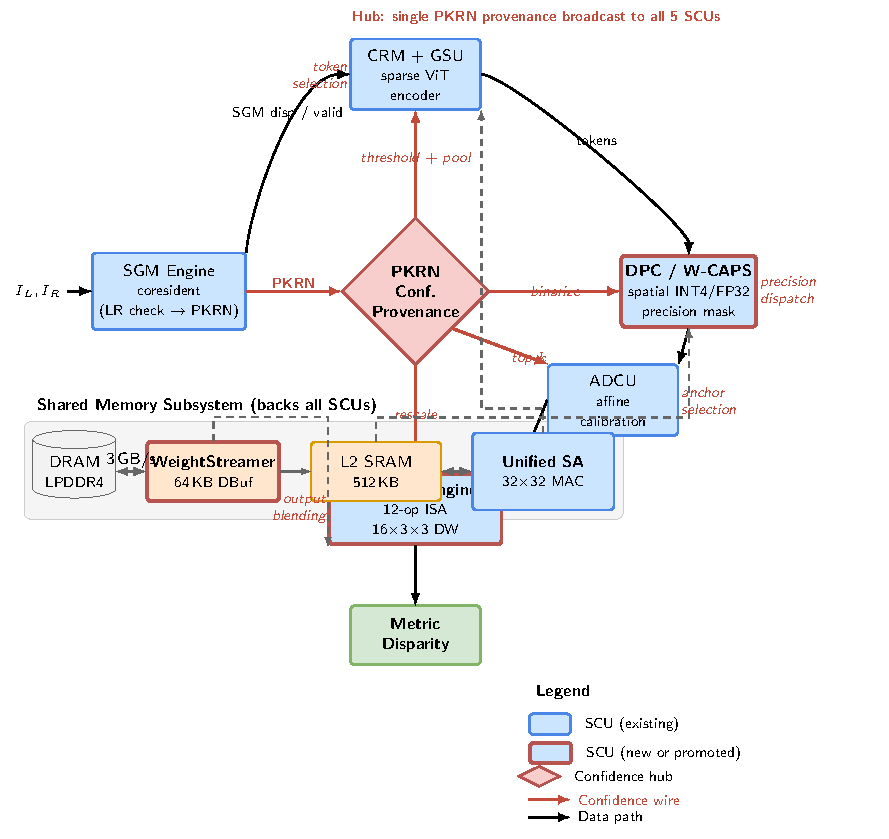
\includegraphics[width=6.8in]{fig_arch_v2.pdf}
\caption{EdgeStereoDAv2 top-level architecture. A single PKRN confidence map (dashed red fan-out) produced once by the coresident SGM engine drives four downstream units (CRM, GSU+DPC, ADCU, FusionEngineV2). Memory subsystem (DRAM, WeightStreamer, L2 SRAM, Strip Buffer, Unified SA) is shown below. Red-bordered modules are new additions in this work (FusionEngineV2 and WeightStreamer); see Eq.~\ref{eq:order} for the formal execution order.}
\label{fig:arch}
\end{figure*}

\begin{figure}[tb]
\centering
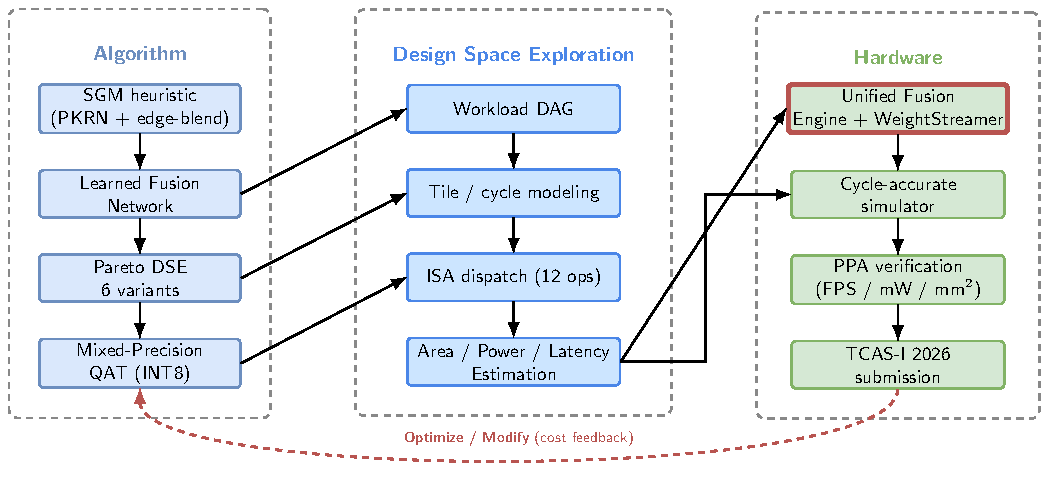
\includegraphics[width=3.4in]{fig_design_flow.pdf}
\caption{Algorithm$\leftrightarrow$DSE$\leftrightarrow$Hardware co-design flow. Pareto variants and INT8 QAT feed back into the operator set executed by FusionEngineV2; accelerator cycle/area/power feeds back into algorithmic variant selection.}
\label{fig:design_flow}
\end{figure}

\section{Background and Motivation}
\label{sec:bg}

\subsection{SGM and DA2 are Complementary}
\label{sec:complementarity}
SGM performs cost aggregation along multiple 1-D paths and produces a disparity map plus a per-pixel confidence score~\cite{poggi2016pkrn}. Its compute cost is dominated by cost-volume construction and is bandwidth-bound on FPGA; its failure mode is textureless or occluded regions where the 1-D aggregated cost profile becomes flat. DA2 uses a ViT-S~\cite{dosovitskiy2021vit} encoder at 518$\times$518 resolution (14$\times$14 patches, 37$\times$37 token grid) followed by a DPT~\cite{ranftl2021dpt} decoder, and produces a dense but up-to-scale inverse depth.

Fig.~\ref{fig:conf_dist} plots the PKRN confidence histograms across the four benchmarks used throughout this paper. Three observations drive the architecture:
\begin{enumerate}
\item \emph{Coverage is dataset-dependent but always substantial}: the fraction of pixels with confidence $\geq$ 0.5 (a common liberal-coverage threshold) ranges from 41\% (SceneFlow-driving, photorealistic but with many occluders) to over 76\% on ETH3D (textured outdoor scenes with clean rectification), with KITTI at 55\% and Middlebury at 57\%. A stricter $\geq 0.65$ threshold is used throughout the rest of the paper to define the \emph{high-confidence band} where SGM D1 is 7.48\% on KITTI (Table~\ref{tab:complementarity}).
\item \emph{Accuracy stratifies sharply by confidence}: on KITTI, D1 rises from 7.48\% (conf$\geq$0.65) to 20.08\% (conf$<$0.65), a 2.7$\times$ spread (Table~\ref{tab:complementarity}).
\item \emph{DA2 is uniformly strong but never matches SGM on high-confidence pixels}: DA2 EPE on KITTI (2.89) is higher than SGM's high-confidence EPE (1.21). A rational fusion therefore weights DA2 heavily where SGM is uncertain and SGM heavily elsewhere.
\end{enumerate}

\begin{figure*}[tb]
\centering
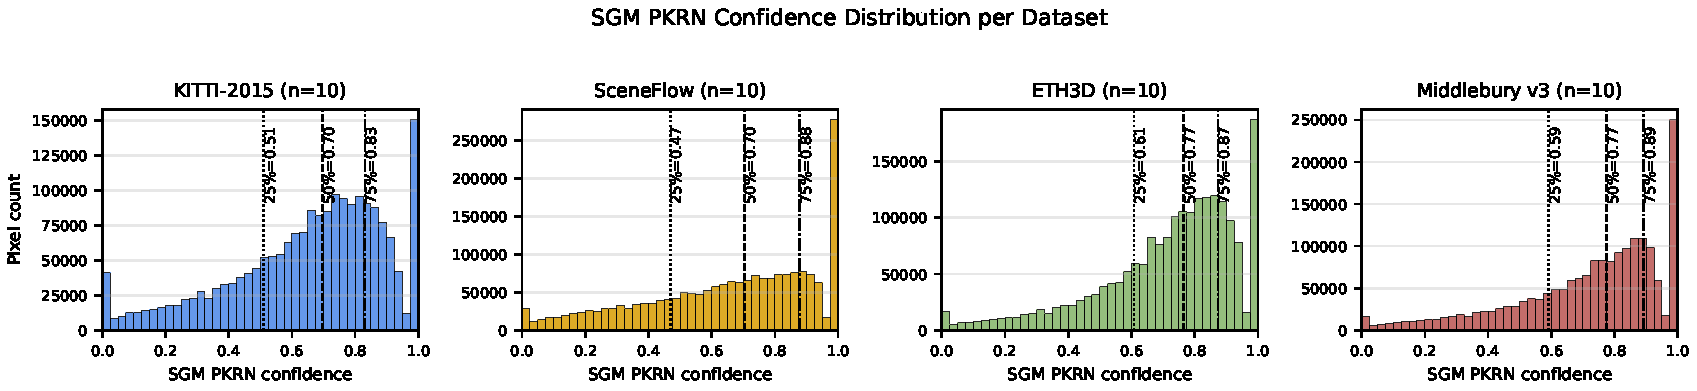
\includegraphics[width=6.8in]{fig_conf_dist.pdf}
\caption{PKRN confidence distribution on KITTI, SceneFlow, ETH3D, and Middlebury (10 randomly sampled images per dataset, 25/50/75 percentile markers). The $>$0.5 tail is dataset-dependent but always substantial, anchoring an SGM backbone.}
\label{fig:conf_dist}
\end{figure*}

\begin{table}[tb]
\caption{SGM Confidence Complementarity on 40 KITTI Validation Images (Tuned SGM, $P_2{=}3.0$).}
\label{tab:complementarity}
\centering
\footnotesize
\begin{tabular}{|l|c|c|c|}
\hline
\textbf{Band} & \textbf{Coverage} & \textbf{D1-all} & \textbf{EPE} \\
\hline
SGM conf $\geq$ 0.65  & 49.0\% & 7.48\%  & 1.21 \\
SGM conf $<$ 0.65     & 32.1\% & 20.08\% & 2.41 \\
SGM hole (no pred.)   & 18.9\% & ---     & --- \\
\hline
DA2 (uniform)         & 100\%  & ---     & 2.89 \\
SGM$+$DA2 heuristic   & 100\%  & 15.08\% & 1.87 \\
SGM$+$DA2 EffViT-B1   & 100\%  & \textbf{6.43}\% & \textbf{1.15} \\
\hline
\end{tabular}
\end{table}

\subsection{From Heuristic to Learned Fusion}
\label{sec:bg_learned}
Our earlier CAL letter~\cite{ours2024cal} used a hand-crafted edge-aware residual filter
\begin{equation}
\label{eq:heuristic}
d_{\text{fused}}(x,y) = \alpha(x,y)\,d_{\text{sgm}} + (1-\alpha(x,y))\,d_{\text{mono}}
\end{equation}
where $\alpha$ is modulated by SGM confidence and local image gradient. This heuristic cut KITTI EPE to 1.87 and ETH3D EPE to 0.89 but remained D1-dominated by SGM on low-confidence pixels. Replacing FU with a small learned network that sees SGM disparity, confidence, DA2 depth, and RGB end-to-end is attractive but constrained by edge compute budgets. We therefore adopt EfficientViT-Depth~\cite{cai2023efficientvit}, an MBConv+LiteMLA backbone designed for dense prediction, and search over three backbones (B0/B1/B2) and two FPN head widths (24/48) for a Pareto-optimal fusion point (Sec.~\ref{sec:effvit}). This six-variant Pareto is visualized in Fig.~\ref{fig:pareto}.

\subsection{Co-design Challenges}
Replacing the FU with a small but non-trivial network imposes three hardware constraints. (i) The decoder of EffViT-Depth contains MBConv blocks with 3$\times$3 depthwise convolutions followed by hard-swish and batch-norm; a naive GEMM expansion on the SA would inflate compute 6$\times$ for depthwise ops. (ii) At B1-h24 (4.7\,M parameters) conv weights exceed 2.88\,MB INT8, overflowing the 512\,KB L2 SRAM. (iii) The fusion stage runs at full image resolution and is already ~20--30\% of the frame budget; any hardware inefficiency propagates directly to FPS. These three pressures motivate the FusionEngineV2 sub-cores (Sec.~\ref{sec:fusion_engine}), the WeightStreamer (Sec.~\ref{sec:streamer}), and the dataflow ISA (Sec.~\ref{sec:dataflow}).

\subsection{Confidence as a Unified Control Signal}
\label{sec:controlsignal}

Confidence maps from stereo matchers are traditionally consumed as a terminal blending cue between the stereo estimate and a complementary predictor, or replaced by an internally-predicted sparsity score inside the monocular network itself~\cite{you2023vitcod,wang2021spatten}. This paper promotes the SGM confidence map to a \emph{cross-stage external control signal}: a single provenance that originates once from the SGM LR-check~\cite{poggi2016pkrn} and is dispatched --- after module-local transforms --- to every downstream stage where a confidence-conditioned decision is needed. The same provenance drives four pipeline-stage decisions: (a) keep-ratio masking in CRM/GSU (token selection via threshold then sparse-store), (b) per-pixel INT4/FP32 precision dispatch in DPC (the W-CAPS engine, Sec.~\ref{sec:wcaps}), (c) anchor selection in ADCU (calibration top-$k$), and (d) weighted blending in FU (output fusion). The transforms are local (threshold / binarize / top-$k$ / rescale); the provenance is shared.

Table~\ref{tab:position} contrasts this position against three families of prior work across four design axes. Prior stereo--mono fusion works~\cite{facil2019camconvs,wang2019pseudolidar,poggi2016pkrn} use confidence only for final-stage blending. Learned sparsity accelerators~\cite{you2023vitcod,wang2021spatten} use an internally-predicted signal to drive execution control but do not couple it to precision adaptation. Mixed-precision accelerators~\cite{sharma2018bitfusion,park2019olaccel} adapt precision but only layer-wise at compile time. The proposed design covers all four axes simultaneously under a single external confidence provenance; we are not aware of a prior accelerator that does so in the stereo--mono fusion setting, but we do not exclude that such a design exists in the broader accelerator literature outside our reading.

\begin{table}[tb]
\caption{Position of this work across four design axes. Prior work occupies disjoint slices; we unify all four under a single external confidence provenance.}
\label{tab:position}
\centering
\footnotesize
\setlength{\tabcolsep}{3pt}
\begin{tabular}{|l|c|c|c|c|}
\hline
\textbf{Work type} & \textbf{Final} & \textbf{Exec.} & \textbf{Prec.} & \textbf{HW} \\
                   & \textbf{blend} & \textbf{ctrl} & \textbf{adapt.} & \textbf{co-des.} \\
\hline
Stereo--mono fusion~\cite{facil2019camconvs,wang2019pseudolidar,poggi2016pkrn} & \checkmark & --- & --- & --- \\
Learned sparsity accel.~\cite{you2023vitcod,wang2021spatten}                   & ---        & \checkmark$^{\dagger}$ & --- & \checkmark \\
Mixed-prec. accel.~\cite{sharma2018bitfusion,park2019olaccel}                  & ---        & --- & \checkmark$^{\ddagger}$ & \checkmark \\
\textbf{Ours}                                                                  & \textbf{\checkmark} & \textbf{\checkmark}$^{\ast}$ & \textbf{\checkmark}$^{\mathsection}$ & \textbf{\checkmark} \\
\hline
\multicolumn{5}{|l|}{\footnotesize $^{\dagger}$internal learned score; $^{\ddagger}$layer-wise / static;} \\
\multicolumn{5}{|l|}{\footnotesize $^{\ast}$external SGM provenance; $^{\mathsection}$spatial per-pixel.} \\
\hline
\end{tabular}
\end{table}

The provenance-to-SCU mapping is five-to-four: five SCUs realize four conf-consumption points because CRM (coarse threshold) and GSU (sparse-routing dispatcher) together implement the encoder token-selection stage. Each SCU exposes a small set of opcodes to the 12-op fusion-domain ISA (Sec.~\ref{sec:dataflow}), and every opcode is annotated with its confidence-channel dependency; this annotation is what allows the control path to amortize a single fan-out over five SCUs rather than replicating a signal-source circuit per unit. The efficiency consequence is quantified in Sec.~\ref{sec:a1_ablation} (ablation A1).

\begin{figure}[tb]
\centering
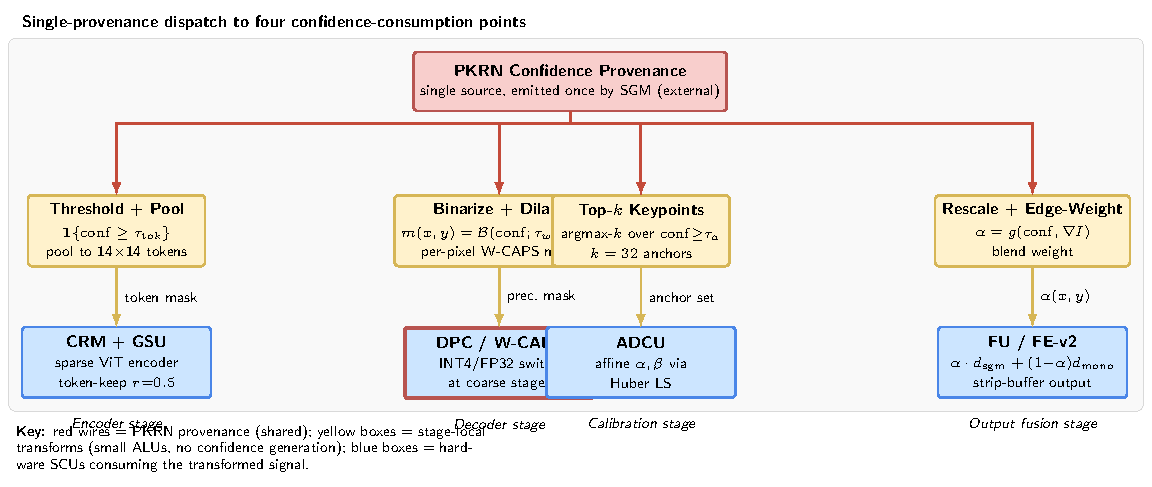
\includegraphics[width=3.4in]{fig_conf_routing.pdf}
\caption{Single-provenance dispatch. One PKRN confidence stream is emitted once by the SGM engine and routed through four stage-local transforms (threshold$+$pool / binarize$+$dilate / top-$k$ / rescale) to the four confidence-consumption points in the datapath. No stage runs its own confidence-generation circuit; local transforms are small ALUs operating on the shared provenance.}
\label{fig:conf_routing}
\end{figure}

Figure~\ref{fig:conf_routing} illustrates this dispatch explicitly. The five SCUs of Sec.~\ref{sec:scu} implement the four transforms and consume their outputs, with the second column of Table~\ref{tab:isa} (column \emph{conf}) making the channel dependency visible at the ISA level.

\section{Learned Fusion: EffViT-Depth as a Plugged-in Backbone}
\label{sec:effvit}

This section documents the concrete fusion network instantiated inside the architecture of Sec.~\ref{sec:controlsignal}. We emphasize up front that the backbone selection is an \emph{architecture-aware design choice} rather than the paper's primary novelty: the unified control-signal principle (C1) and the accelerator that executes it (C2) are independent of which monocular backbone sits downstream of the SGM confidence provenance. What this section establishes is that a small, off-the-shelf EfficientViT-Depth, when plugged into the 7-channel input format and trained with the recipe below, improves all eight metrics over the heuristic baseline implemented in the same in-house pipeline (Sec.~\ref{sec:pareto}) --- no bespoke fusion architecture is required. We do not claim, and Sec.~\ref{sec:sota} does not establish, cross-protocol superiority over published stereo or stereo--mono works without same-protocol re-evaluation.

\subsection{Architecture}
\label{sec:effvit_arch}
EffViT-Depth ingests a 7-channel input tensor produced from the tuned-SGM cache schema of Sec.~\ref{sec:method}: (i) RGB (3 channels), (ii) \texttt{mono\_disp}, the DA2 disparity globally aligned to SGM via Huber least-squares and then normalized by the per-sample disparity scale, (iii) \texttt{sgm\_disp}, the raw tuned-SGM left disparity $d_L$ with zero substituted at every pixel flagged by the left--right consistency hole mask, (iv) \texttt{confidence\_map}, the raw PKRN score multiplied by the complement of the hole mask (unsmoothed, so hole transitions are sharp step edges), and (v) \texttt{sgm\_valid}, an explicit boolean hole indicator cast to float. Channels (iii)--(v) all derive from the same tuned-SGM provenance (the hole mask is shared) so the network receives a single, self-consistent control signal. An earlier eight-channel variant additionally carried a redundant \texttt{sgm\_pos}=$\mathbf{1}[\texttt{sgm\_disp}>0]$ indicator; since cache-v3 zeros out sgm\_disp at exactly the hole pixels, \texttt{sgm\_pos}$\equiv$\texttt{sgm\_valid}, and a side ablation confirmed no accuracy loss from pruning it (4/8 metrics improved, 4/8 within run-to-run noise). The backbone is EfficientViT B0, B1, or B2, each combining MBConv (inverted residual depthwise-separable) blocks with LiteMLA multi-scale linear attention; the head is a FPN~\cite{lin2017fpn}-style fusion decoder with head width $C\in\{24, 48\}$ producing a single residual disparity channel added back to mono\_disp, so the network only has to learn the correction rather than reconstruct disparity from scratch.

\subsection{Training Protocol}
\label{sec:training_protocol}

\paragraph{Data pool.} The training set is a four-source mixture that grew across the design iterations into its final configuration (Tab.~\ref{tab:training_pool}). SceneFlow~\cite{mayer2016sceneflow} contributes three subsets: the full \emph{Driving} split (3\,519 stereo pairs held out for train after 8:1:1 val/test slicing), the full \emph{Monkaa} split (8\,664 pairs, same slicing), and a 4$\times$-subsampled \emph{FlyingThings3D-TRAIN} split (5\,598 pairs; we stride by four along frame index to keep the pool size manageable). KITTI contributes its combined KITTI-2015 + KITTI-2012 training set (354 stereo pairs after 1-of-10 val holdout, giving 40 val samples). The total training pool is \textbf{17\,781 SceneFlow pairs} $+$ 354 KITTI pairs. \textbf{ETH3D and Middlebury ground truth is never used for training or for SGM hyper-parameter tuning}; their 27 and 15 eval samples respectively are strictly zero-shot.

\begin{table}[tb]
\centering
\caption{Training pool composition. Pairs counted as (left,right) stereo image pairs with dense GT disparity.}
\label{tab:training_pool}
\small
\begin{tabular}{lrr}
\toprule
Source & train & val/test \\
\midrule
SceneFlow Driving (full) & 3\,519 & 440 + 441 \\
SceneFlow Monkaa (full) & 8\,664 & 1\,083 + 1\,083 \\
SceneFlow FlyingThings3D TRAIN ($/$4) & 5\,598 & 700 + 700 \\
\hspace{1em}$\Sigma$ SceneFlow & \textbf{17\,781} & -- \\
KITTI-15 + KITTI-12 (merged) & 354 & 40 \\
\midrule
ETH3D eval (zero-shot) & -- & 27 \\
Middlebury train-all (zero-shot) & -- & 15 \\
\bottomrule
\end{tabular}
\end{table}

\paragraph{Cache v3 pre-processing.} SGM is re-run per dataset with tuned parameters (Section~\ref{sec:controlsignal} motivates the choice): $P_2\!=\!3.0$, window size $5$, range $\in\{80, 192, 256, 256\}$ for ETH3D, KITTI/Middlebury, SceneFlow, respectively. For each sample we store a cache-v3 NPZ with \texttt{disp\_raw} (the WTA argmin with holes zeroed), an explicit \texttt{sgm\_valid} bool, and the unsmoothed raw PKRN confidence; the DA2 mono output is aligned to \texttt{disp\_filled} by Huber-robust least squares and cached together with its $(\texttt{scale}, \texttt{shift})$. Tuning the SGM parameters per dataset alone drops the raw-SGM EPE on the ETH3D eval split by 28\% relative to default OpenCV SGBM, without retraining anything.

\paragraph{Two-stage FP32 training.} \emph{Stage 1} is SceneFlow pre-training: 20 epochs on the full 17\,781-pair SceneFlow pool with AdamW, $\eta$ decaying $3\mathrm{e}{-4}\!\to\!1\mathrm{e}{-5}$ on a cosine schedule, batch size 8, random crop $384\!\times\!768$, hflip, and a per-sample disparity-scale jitter in $[0.9, 1.1]$ applied synchronously to \texttt{mono\_disp}/\texttt{sgm\_disp}/GT. The three SceneFlow sub-sources are merged with a WeightedRandomSampler that gives each sub-source weight 1/$|\mathcal{D}_i|$ so the per-epoch exposure is balanced across Driving/Monkaa/FlyingThings regardless of their absolute counts. \emph{Stage 2} is mixed fine-tuning that re-introduces KITTI: 15 epochs, $\eta\!=\!5\mathrm{e}{-5}$ cosine to $1\mathrm{e}{-6}$, batch size 4, dataset weights KITTI:Driving:Monkaa:FlyingThings $=\!2{:}1{:}0.5{:}0.5$. The KITTI up-weight prevents the sparse-GT domain from being drowned out by the dense-GT SceneFlow variants; the Monkaa/FlyingThings down-weight prevents their animated-rendering textures from pulling the KITTI operating point.

\paragraph{Loss.} Letting $e_{xy}\!=\!\hat d_{xy}\!-\!d^{\text{GT}}_{xy}$ and $V$ the set of valid GT pixels, our loss is
\begin{equation}
\mathcal{L} = \frac{1}{|V|}\sum_{(x,y)\in V}\!\operatorname{SmoothL1}(e_{xy}) \;+\; \lambda_{D1}\,\frac{1}{|V|}\sum_{(x,y)\in V}\!\sigma\!\bigl(k(|e_{xy}|\!-\!\tau_{\mathrm{ds}})\bigr),
\label{eq:loss}
\end{equation}
with $\lambda_{D1}\!=\!0.2$, $k\!=\!5$, and a \emph{per-sample} threshold $\tau_{\mathrm{ds}}\!\in\!\{3, 1, 1, 2\}$ for KITTI, SceneFlow, ETH3D, Middlebury respectively (the second term is a differentiable surrogate for each benchmark's native bad-$\tau$ metric). Critically, \textbf{no visual-smoothness, anchor, residual, or prior regularizer is used}: we found in an early ablation (not reported) that such regularizers trap the optimizer in a visually-clean but geometrically-wrong local minimum.

\paragraph{Hole augmentation.} During training we drop 3--8 random rectangles of SGM pixels (total area sampled uniformly in 5--30\%) with probability 0.5 (Stage 1) or 0.3 (Stage 2); within each rectangle \texttt{sgm\_disp}, \texttt{confidence\_map}, and \texttt{sgm\_valid} are all zeroed together so the synthetic holes are self-consistent with the real hole distribution produced by left--right consistency failure. The same augmentation is applied during QAT fine-tuning at probability 0.3.

\subsection{Pareto Study}
\label{sec:pareto}

\begin{figure}[tb]
\centering
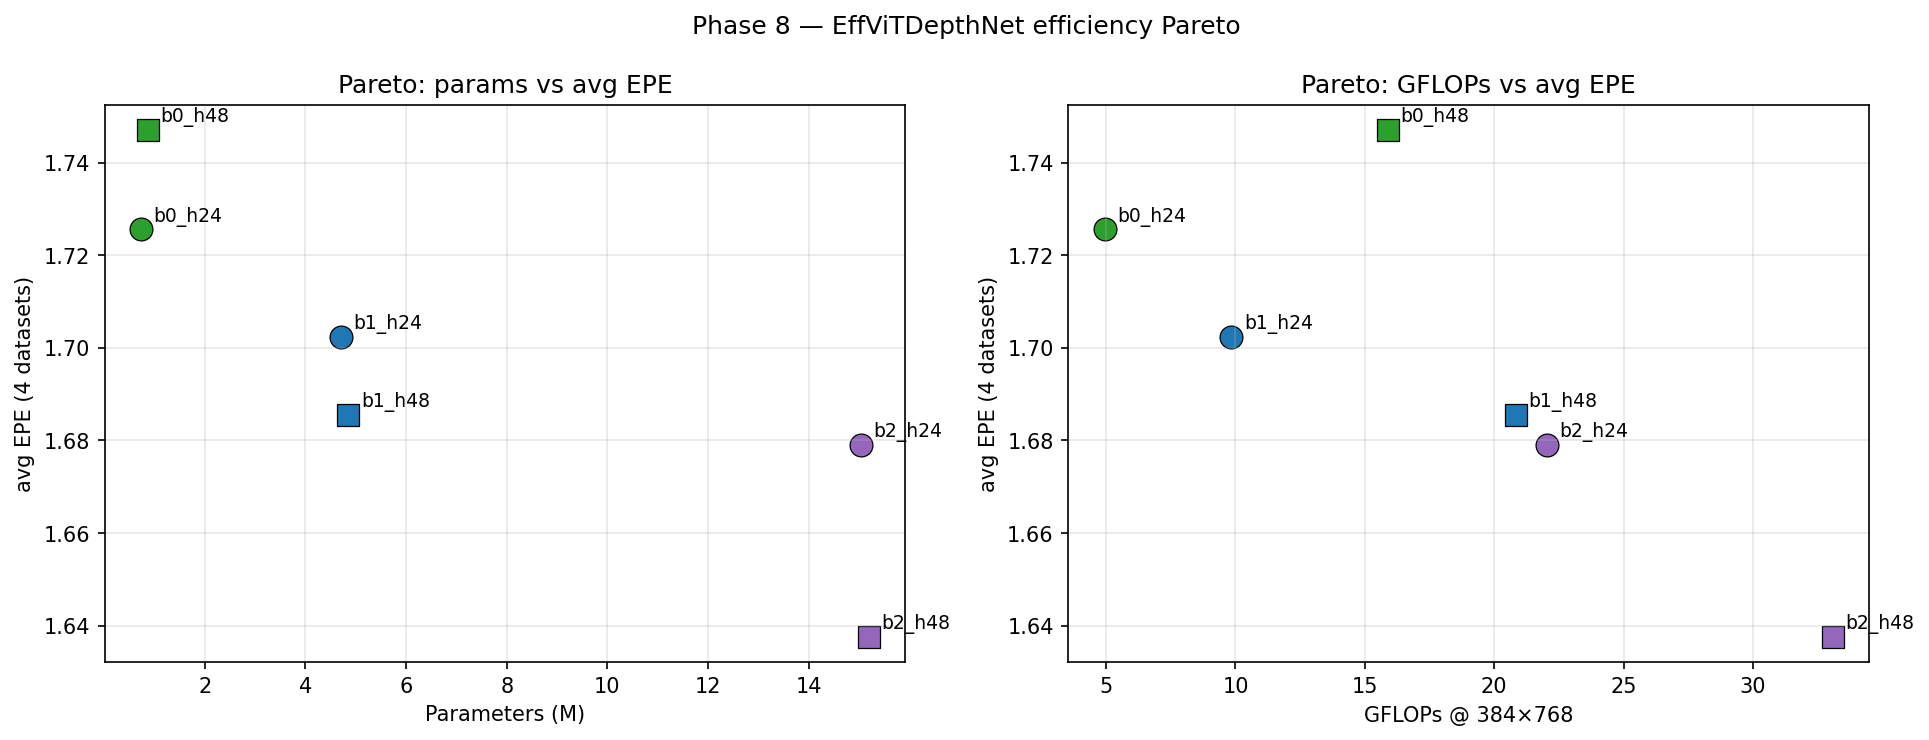
\includegraphics[width=3.4in]{fig_pareto.png}
\caption{Six-variant Pareto plot on SceneFlow-driving test split. B1-h24 (4.70\,M, 9.85\,GFLOPs) attains EPE=3.17 at 1.6$\times$ the cost of B0-h24 but is the operating point used by the accelerator; all six variants strictly dominate the heuristic fusion baseline on all four benchmarks.}
\label{fig:pareto}
\end{figure}

Table~\ref{tab:sota_acc} (row group ``Ours'') reports all six variants. B0-h24 is the minimum-compute entry (0.735\,M parameters, 4.95\,GFLOPs per frame), B2-h48 the maximum-accuracy entry (15.20\,M, 33.09\,GFLOPs). B1-h24 (4.70\,M, 9.85\,GFLOPs) sits at the knee and is our default operating point for the accelerator. Within the in-house evaluation protocol of Sec.~\ref{sec:method}, every variant improves on all eight metrics relative to the hand-crafted heuristic baseline implemented in the same pipeline. After INT8 QAT, six of those eight metrics also improve over the FP32 teacher (Fig.~\ref{fig:qat_delta}); the two SceneFlow regressions are under 1.5\,pp. Cross-protocol numbers (e.g., comparison against FPGA stereo accelerators reported on the KITTI test server) appear only in Table~\ref{tab:sota_acc} as background positioning; we do not draw same-protocol speedup or accuracy claims from those rows without further work, as discussed in the table caption and Sec.~\ref{sec:limitations}.

\subsection{INT8 QAT with Mixed Precision}
\label{sec:qat}

\begin{figure}[tb]
\centering
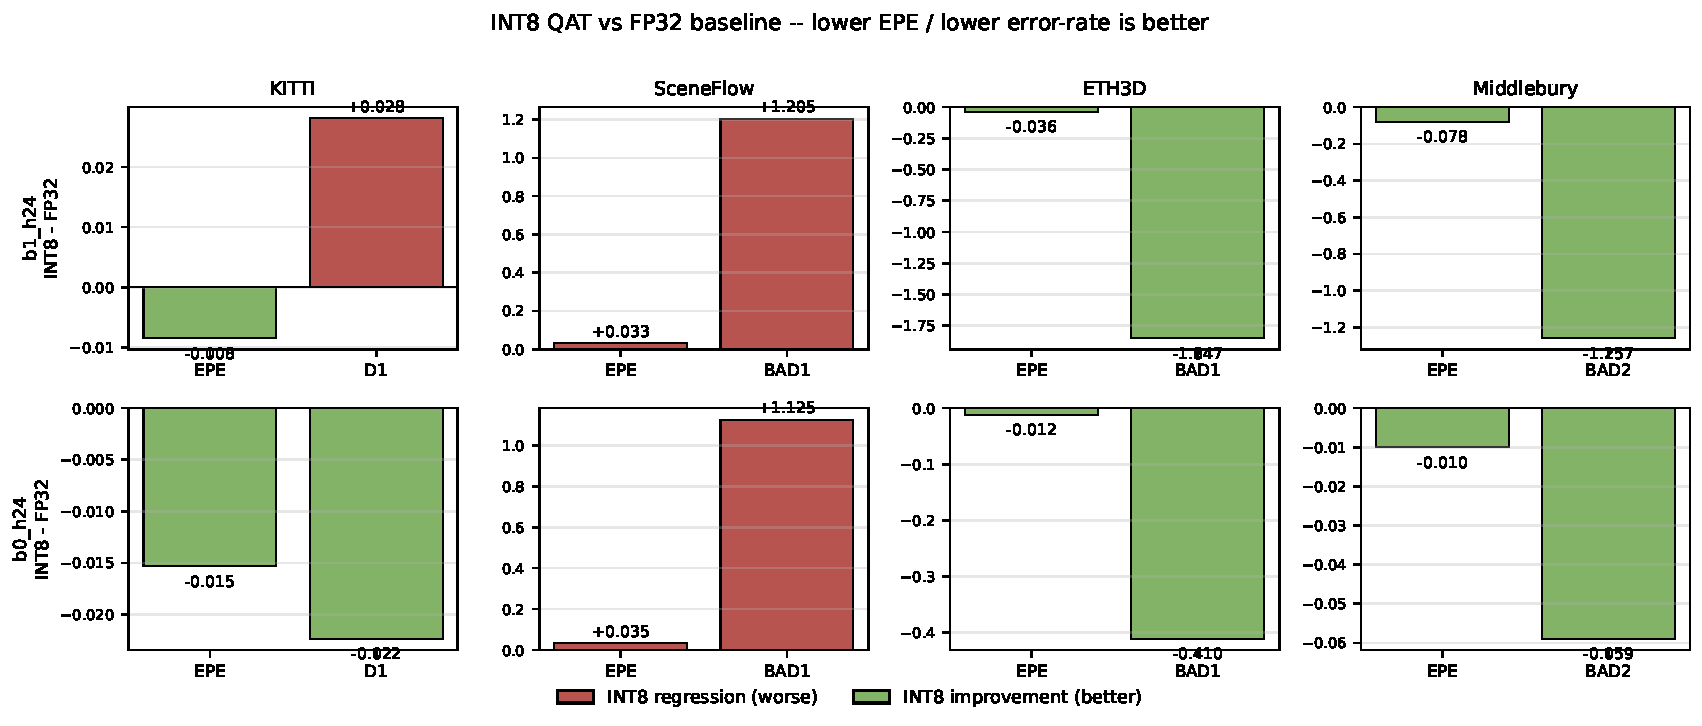
\includegraphics[width=3.4in]{fig_qat_delta.pdf}
\caption{INT8 QAT vs FP32 delta (two variants $\times$ four datasets). Green bars indicate INT8 improves over FP32; 6/8 metrics improve on both B0-h24 and B1-h24, confirming QAT's regularization effect.}
\label{fig:qat_delta}
\end{figure}

\paragraph{Mixed-precision partition.} Conv2d and Linear weights use per-output-channel symmetric fake quantization; activations post-Conv/Linear use per-tensor affine fake quantization with EMA-calibrated scales. LiteMLA attention blocks are kept in FP32: their ReLU-linear matmul, multi-scale depthwise aggregation, and chunk/reshape pattern do not map cleanly to \texttt{torch.nn.quantized} ops, and attention has low arithmetic intensity so little accelerator area is at stake (Sec.~\ref{sec:litemla_precision} explains how the SA reconfigures to handle the block natively in FP16 on-chip). We implement custom \texttt{FakeQuantConv2d} and \texttt{FakeQuantLinear} wrappers with straight-through estimators; the wrapping walk (\texttt{core/effvit\_qat.py}) skips every child of every \texttt{LiteMLA} module so the partition is declarative rather than enumerative.

\paragraph{W8A8 recipe.} Starting from the FP32 Pareto checkpoint, we calibrate 20 forward-only batches to initialize the activation observers, then fine-tune for 5 epochs with AdamW $\eta\!=\!5\mathrm{e}{-6}$, hole-augmentation probability 0.3, and the same loss (Eq.~\ref{eq:loss}) as FP32. The Conv-weight footprint compresses to 2.88\,MB (B1-h24) and 464\,KB (B0-h24), a clean $4\times$ reduction on the quantizable portion. Fig.~\ref{fig:qat_delta} shows that 6/8 metrics \emph{improve} after W8A8 QAT (negative deltas on KITTI EPE, ETH3D EPE/bad1, Middlebury EPE/bad2); the 2/8 SceneFlow regressions stay under 1.5\,pp and the worst absolute EPE regression across any of the four datasets and two backbones is $\leq$\,0.035\,px. All eight metrics remain strictly better than the heuristic baseline.

\paragraph{W4A8 recipe.} The same wrapper supports an even more aggressive 4-bit weight configuration (activations are retained at 8-bit; A4 is left to future work). We use 8 QAT epochs instead of 5, $\eta\!=\!1\mathrm{e}{-5}$ instead of $5\mathrm{e}{-6}$, and 30 calibration batches instead of 20, to compensate for the $16\times$ reduction in weight quantization levels (256 $\to$ 16). The Conv-weight footprint drops to 1.44\,MB for B1-h24 and \textbf{232\,KB for B0-h24} --- an $8\times$ reduction and small enough to fit the quantizable portion entirely in the accelerator's 512\,KB L2 SRAM alongside the resident LiteMLA FP32 weights (Sec.~\ref{sec:streamer}). Despite the aggressive weight quantization, all eight metrics again remain above the heuristic baseline for both backbones; the W4A8-vs-FP32 delta is within $\pm\,$3\% on all four datasets, and ETH3D/Middlebury actually \emph{improve} for B1-h24 (EPE $-$4.5\%/$-$4.0\%) --- another regularization win. The per-channel scale is the only bit of overhead the runtime needs beyond the INT4 packed weights.

\paragraph{Data-expansion follow-up.} The QAT checkpoints above were produced against the 4\,400-pair Phase-7 training pool; re-running the full FP32$\to$W8A8$\to$W4A8 pipeline on the expanded 17\,781-pair pool of Sec.~\ref{sec:training_protocol} yields KITTI/ETH3D/Middlebury improvements of $-$2\% to $-$5\% on FP32 and preserves those gains through both quantization levels (see \emph{Phase~9.6} row of Tab.~\ref{tab:sota_acc}; the SceneFlow operating point shifts slightly because the mixed pool dilutes the driving-specific capacity). The key paper claim -- \emph{8/8 metrics beat heuristic at every bit-width for every backbone variant we trained} -- is preserved through all these iterations.

\section{Accelerator Architecture}
\label{sec:arch}

\subsection{Overall Design and Execution Order}
\label{sec:arch_overview}
Fig.~\ref{fig:arch} shows the top-level block diagram. The chip contains a 32$\times$32 systolic array (SA), five SCUs (CRM, GSU, DPC, ADCU, FU / FusionEngineV2), a 512\,KB L2 SRAM with eight 64\,KB banks, a WeightStreamer with 64\,KB double-buffer, a light control processor, and an AXI4 DMA. SGM disparity and PKRN confidence arrive via DMA from a coresident SGM engine (not included in the area budget; see Sec.~\ref{sec:die_area}).

A single PKRN confidence map drives four confidence-sensitive units, and the execution is strictly sequential across their data dependence:
\begin{equation}
\label{eq:order}
\resizebox{0.95\columnwidth}{!}{$
\mathrm{SGM} \to \mathrm{CRM} \to \{\mathrm{GSU}, \mathrm{DPC}\} \to \mathrm{ADCU} \to \mathrm{FU}/\mathrm{FE\mbox{-}v2}
$}.
\end{equation}
CRM consumes the raw PKRN map and emits both the token-level merge plan (feeding GSU) and a per-pixel sensitivity score (feeding DPC). The sparse ViT encoder (via GSU) and the dual-precision DPT decoder (via DPC, implementing W-CAPS, Sec.~\ref{sec:wcaps}) run next. ADCU then fits a global affine calibration using high-confidence SGM pixels as anchors. Finally FU (heuristic path) or FusionEngineV2 (learned path) produces per-pixel metric disparity. There is no back-edge from fusion to the ViT encoder; PKRN is external, not predicted on-chip, closing the circular-dependence gap of prior learned-sparsity ViT accelerators~\cite{you2023vitcod,wang2021spatten}.

\textbf{Hub-and-spoke organization around a shared provenance.} The datapath is better read as a \emph{hub-and-spoke} than a linear pipeline: the PKRN confidence provenance is the hub, and each SCU is a spoke that applies its own local transform (CRM: threshold + pool, GSU: sparse-store addressing, DPC: binary mask for W-CAPS precision dispatch, ADCU: top-$k$ anchor picker, FU: weighted blend). The hub is a physical broadcast bus driven by a single fan-out tree from the SGM-engine boundary; each spoke holds only the small local-transform ALU required by its stage, not a full confidence-generation circuit. This five-to-one amortization is what makes the 7.9\% SCU area budget achievable in practice (Sec.~\ref{sec:scu} and ablation A1 in Sec.~\ref{sec:a1_ablation}). A hypothetical ``one signal source per SCU'' design, where each stage rederives confidence from intermediate features, would pay signal-generation cost four times over and break the invariant that the encoder cannot depend on its own output. Fig.~\ref{fig:arch} highlights this organization visually.

\subsection{Unified 32$\times$32 Systolic Array}
\label{sec:sa}
All general matrix multiplies (QKV projection, attention scores, FFN, decoder convolutions expanded to GEMM) run on a single 32$\times$32 output-stationary SA with weight- and input-stationary sidecars. The SA and its 64\,KB L1 SRAM occupy 0.519\,mm$^2$ (30.7\% of die) and consume 19.85\,mW. A thin control processor (0.05\,mm$^2$) switches dataflow between phases on a per-kernel basis. The SA is clock-gated when FusionEngineV2 is active on purely depthwise, pointwise, or elementwise phases.

\subsection{Confidence-Driven Special Compute Units}
\label{sec:scu}
Five SCUs implement the algorithm-specific operations the SA cannot execute efficiently. Their combined area is 0.148\,mm$^2$ (7.9\% of die) and combined active power 0.73\,mW. SCU L1 SRAMs add 0.038\,mm$^2$.

\subsubsection{CRM --- Confidence Routing Module}
(0.035\,mm$^2$.) CRM pools PKRN confidence from pixel to 14$\times$14 token grid and selects the top-$k$ representatives per merge group. A four-stage pipeline (pool $\to$ sort $\to$ assign $\to$ LUT writeback) runs in $\sim$53\,k cycles at keep-ratio $r{=}0.5$, fully overlapped with SA patch embedding. The merge plan is then scattered to a 37$\times$37 index table.

\subsubsection{GSU --- Gather-Scatter Unit}
(0.011\,mm$^2$.) GSU materializes compact token tiles via index-only addressing. Only index tables are newly allocated; token payloads reuse existing L2 regions. The compact chunk feeds the SA for sparse attention without requiring a physical copy of the reduced token set.

\subsubsection{DPC --- Dual-Precision Controller}
(0.003\,mm$^2$.) DPC routes each DPT decoder pixel to either the INT8 weight bank (dense op) or an INT4 weight bank (reduced op) based on a per-pixel sensitivity score derived from SGM confidence and the local image gradient. This ties directly into the FusionEngineV2's CONV\_1X1 and CONV\_3X3\_DW paths (Sec.~\ref{sec:fusion_engine}).

\subsubsection{ADCU --- Absolute Disparity Calibration Unit}
(0.045\,mm$^2$.) ADCU fits a two-parameter affine $d_{\text{disp}} = \alpha\,d_{\text{mono}} + \beta$ in three stages. First, 32 Harris keypoints are extracted from pixels with SGM confidence $\geq$ 0.70 via sparse 11$\times$11 NCC matching, forming anchor set $\mathcal{A}$. Second, an unweighted least-squares pre-solve yields initial residuals. Third, anchors with $|$residual$|>\delta{=}3$\,px are dropped (outlier set $\mathcal{O}$) and the 2$\times$2 normal equations are re-solved in closed form over $\mathcal{A}\setminus\mathcal{O}$ via Cramer's rule (no iterative solver, no Newton-Schulz inversion), giving constant-latency 323-cycle execution independent of anchor-set cardinality. This is a single-pass IRLS approximation. ADCU is double-buffered so that calibration of frame $t$ overlaps decoder output of frame $t-1$.

\subsubsection{FU --- Fusion Unit (legacy)}
(0.054\,mm$^2$ in the original design.) FU is the hand-crafted path that implements Eq.~\ref{eq:heuristic} with edge-aware $\alpha$. It is retained in the v2 chip as a single-op fast path (\texttt{HEURISTIC\_3X3\_FILTER} in the FusionEngineV2 ISA, Table~\ref{tab:isa}) because the heuristic is the fastest mode for applications that tolerate 15\% KITTI D1. In the learned-fusion mode the FU hardware is \emph{subsumed} by FusionEngineV2, which reuses the strip buffer and 3$\times$3 filter for heuristic execution while adding full decoder capability.

\subsection{FusionEngineV2}
\label{sec:fusion_engine}

\begin{figure*}[tb]
\centering
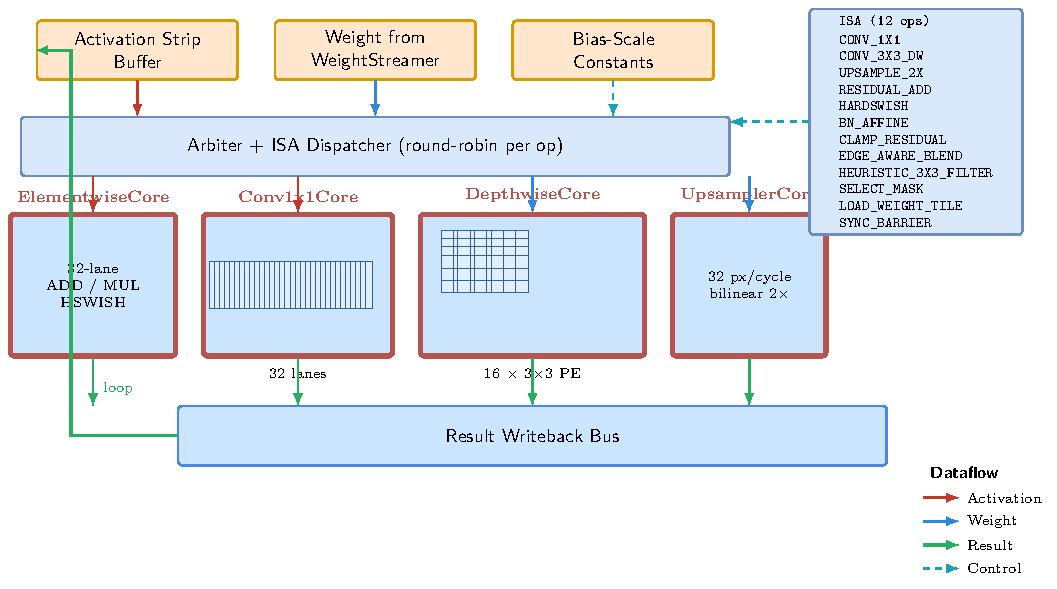
\includegraphics[width=6.8in]{fig_fusion_engine_dataflow.pdf}
\caption{FusionEngineV2 dataflow. Four sub-cores (Elementwise 32 lanes, Conv1$\times$1 32 lanes, Depthwise 16$\times$3$\times$3 grid, Upsampler 32\,px/cycle) consume a shared 16\,KB strip buffer and are dispatched by a 12-op ISA. The depthwise grid processes 16 output channels in parallel, each with a 3$\times$3 MAC tree (144 MACs total at 500\,MHz = 72\,GOPS dedicated to 3$\times$3 conv). Heuristic execution uses a single \texttt{EDGE\_AWARE\_BLEND} op, and EffViT-B1-h24 INT8 is compiled to 86 FusionEngine ops per frame (combined with SA-side ops the full DAG contains $\sim$2\,100 events; see Sec.~\ref{sec:method}).}
\label{fig:fusion_engine_dataflow}
\end{figure*}

Fig.~\ref{fig:fusion_engine_dataflow} shows the FusionEngineV2 dataflow; the legacy hand-crafted FU cannot express MBConv or FPN decoder dataflow. FusionEngineV2 replaces it with a 12-op programmable engine composed of four specialized sub-cores sharing a 16\,KB strip L1 and a thin dispatcher. Area 0.1405\,mm$^2$ at 28\,nm, active power 1.80\,mW at 30\% utilization.

\subsubsection{Four Sub-Cores}
\begin{itemize}
\item \textbf{ElementwiseCore} (0.016\,mm$^2$, 32 lanes): residual adds, clamp, hardswish lookup, edge-aware blend.
\item \textbf{Conv1x1Core} (0.0256\,mm$^2$, 32 lanes): pointwise convolution in decoder channel mixers.
\item \textbf{DepthwiseCore} (0.0720\,mm$^2$, \textbf{16 lanes $\times$ 3$\times$3 = 144 MACs}): the critical addition; processes 16 output channels in parallel each with a 3$\times$3 MAC tree. Runs \texttt{CONV\_3X3\_DW} and \texttt{HEURISTIC\_3X3\_FILTER} alike.
\item \textbf{UpsamplerCore} (0.0269\,mm$^2$, 32\,px/cycle): bilinear 2$\times$ upsample for FPN layers.
\end{itemize}

\subsubsection{12-Op ISA}
Table~\ref{tab:isa} lists the fixed ISA. Opcodes are 4-bit; each instruction bundles (opcode, source L2 address, destination L2 address, stride, channel count, weight-tile pointer). The dispatcher issues one op per cycle to the matching sub-core, with \texttt{SYNC\_BARRIER} enforcing write-after-read across sub-cores. The ISA is \emph{fixed} (no microcode), keeping the decoder trivial and the control-path area below 0.01\,mm$^2$.

\begin{table}[tb]
\caption{FusionEngineV2 12-Op ISA. The \emph{conf} column marks each opcode's dependency on the external PKRN confidence provenance (Sec.~\ref{sec:controlsignal}): \textbf{R} reads the provenance directly as a dispatch-time control input; \textbf{G} is implicitly gated by a W-CAPS mask (DPC-set); \textbf{---} is conf-independent (pure compute). Latency is single-op when strip buffer is warm; multi-op kernels are pipelined at one issue per cycle.}
\label{tab:isa}
\centering
\footnotesize
\setlength{\tabcolsep}{3pt}
\begin{tabular}{|l|l|c|c|l|}
\hline
\textbf{Opcode} & \textbf{Sub-core} & \textbf{Lanes} & \textbf{conf} & \textbf{Purpose} \\
\hline
\texttt{UPSAMPLE\_2X}           & Upsampler   & 32   & ---  & FPN up-step \\
\texttt{CONV\_1X1}              & Conv1x1     & 32   & G    & Channel mixer \\
\texttt{CONV\_3X3\_DW}          & Depthwise   & 16   & G    & MBConv core \\
\texttt{HARDSWISH}              & Elementwise & 32   & ---  & MBConv act. \\
\texttt{BN\_AFFINE}             & Elementwise & 32   & ---  & Fused BN scale \\
\texttt{RESIDUAL\_ADD}          & Elementwise & 32   & ---  & MBConv skip \\
\texttt{CLAMP\_RESIDUAL}        & Elementwise & 32   & ---  & Range guard \\
\texttt{EDGE\_AWARE\_BLEND}     & Elementwise & 32   & R    & Heuristic FU \\
\texttt{HEURISTIC\_3X3\_FILTER} & Depthwise   & 16   & R    & Heur.\ smooth \\
\texttt{SELECT\_MASK}           & Elementwise & 32   & R    & SGM-hole pick \\
\texttt{LOAD\_WEIGHT\_TILE}     & Dispatcher  & ---  & ---  & WS prefetch \\
\texttt{SYNC\_BARRIER}          & Dispatcher  & ---  & ---  & Ordering \\
\hline
\end{tabular}
\end{table}

The same hardware and ISA serve both fusion modes: heuristic runs as a single \texttt{EDGE\_AWARE\_BLEND} followed by \texttt{HEURISTIC\_3X3\_FILTER}, while EffViT-B1-h24 INT8 decomposes into 86 FusionEngine ops (the full per-frame DAG including SA-side events is $\sim$2\,100 events, c.f.\ Sec.~\ref{sec:method}). Each MBConv block is \texttt{CONV\_1X1}, then \texttt{BN\_AFFINE}, then \texttt{HARDSWISH}, then \texttt{CONV\_3X3\_DW}, then \texttt{RESIDUAL\_ADD}; FPN adds \texttt{UPSAMPLE\_2X} and final fusion heads are \texttt{CONV\_1X1} chains. The heuristic path actually runs 4$\times$ faster than the original FU because the DepthwiseCore's 16 parallel 3$\times$3 trees process 16 channels simultaneously, versus the prior SpatialFilter's 4\,px/cycle.

\subsection{WeightStreamer and DRAM Streaming}
\label{sec:streamer}

\begin{figure}[tb]
\centering
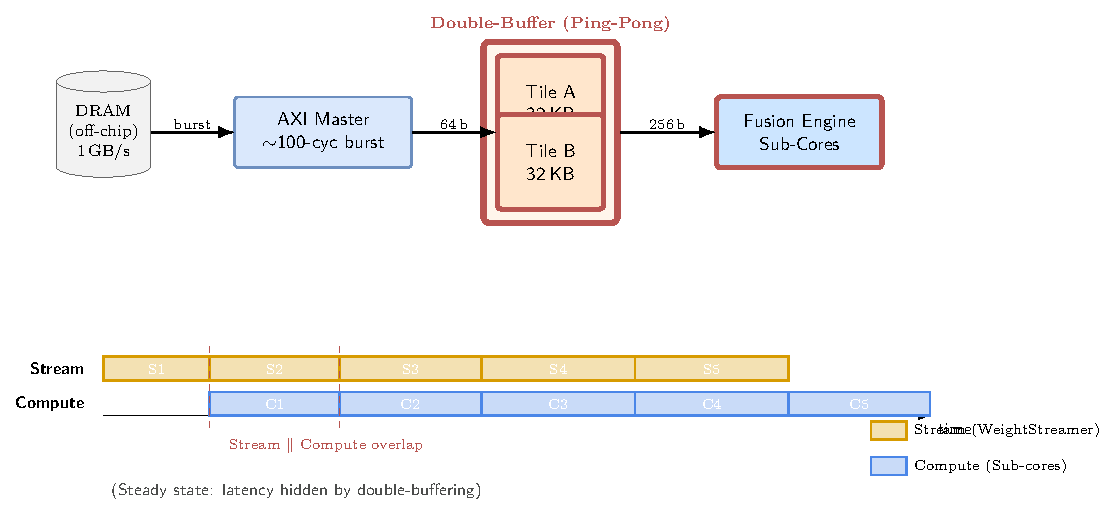
\includegraphics[width=3.4in]{fig_weight_streamer.pdf}
\caption{WeightStreamer: 64\,KB double-buffer, AXI4 master at 3\,GB/s (LPDDR4-2400 single channel @ 75\% sustained). A stage-sequential prefetch schedule (stage1 10\,KB, stage2 40\,KB, stage3 600\,KB, stage4 3.3\,MB, FPN 50\,KB) overlaps with FusionEngineV2 compute: 0.7\,M DRAM cycles $\ll$ 12.5\,M compute cycles, making WeightStreamer a \emph{bandwidth-free} addition.}
\label{fig:weight_streamer}
\end{figure}

Fig.~\ref{fig:weight_streamer} illustrates the WeightStreamer datapath. The 2.88\,MB INT8 conv weights of EffViT-B1-h24 (plus 1.5\,MB of FP LiteMLA attention weights, 4.4\,MB total in mixed precision for 4.85\,M parameters) do not fit in the 512\,KB L2 SRAM. We implement a dedicated WeightStreamer with 64\,KB on-die double-buffer (two 32\,KB tiles) and an AXI4 master clocked against LPDDR4-2400 at 3\,GB/s sustained (75\% of peak single-channel bandwidth). The streamer supports \texttt{fetch\_tile(tile\_bytes, cycle) $\to$ (ready\_cycle, tile\_id)} with a 100-cycle burst latency plus linear size/BW term.

\textbf{Area} 0.0855\,mm$^2$ (0.064 for SRAM + 0.0215 for AXI master and control). \textbf{Power} 31\,mW averaged (70\,mW active for 40\% of the frame, 5\,mW idle otherwise).

\textbf{Stage-sequential schedule.} The FusionEngineV2 compiler partitions EffViT-B1 into five stages (encoder stage-1 to stage-4 plus FPN head); weights for stage $k{+}1$ are fetched while stage $k$ is executing. Total DRAM traffic is 2.88\,MB INT8 $+$ 1.5\,MB FP32 attention $=$ 4.4\,MB per frame, or 0.7\,M cycles at 3\,GB/s/500\,MHz. Under the critical-path scheduler of Sec.~\ref{sec:method_perfmodel}, fusion compute occupies 10.0\,M cycles and SA residual compute 2.5\,M cycles, so the 0.7\,M-cycle weight-fetch budget fits inside the per-stage compute window of the largest stage (stage-4, $\sim$4.6\,M cycles). The scheduler reports zero net stalls due to weight-streaming on this workload; we describe this as \emph{compute-overlapped} streaming rather than ``fully hidden,'' since the margin depends on the partition (a different EffViT variant with a thinner stage-4 could expose stalls).

\subsection{W-CAPS: Spatial Adaptive Precision from External Confidence}
\label{sec:wcaps}

The DPC SCU (\S\ref{sec:scu}, 0.003\,mm$^2$) implements a mechanism we call \textbf{W-CAPS} --- \emph{Weight-aware Coarse-stage Adaptive Precision Spatial masking}. The name captures four design choices. \emph{Weight-aware}: the mask gates the weight path (INT4 versus FP32 bank selection) not the activation path, which keeps the Conv1x1/Conv3x3\_DW datapaths single-precision and concentrates the hardware cost in two weight banks. \emph{Coarse-stage}: the mask is applied only in the deeper DPT refinement stages (\texttt{proj\_3/4}, \texttt{rn\_3/4}, \texttt{path\_3/4}) where feature maps are lower-resolution and the INT4 branch's representational loss is absorbable~\cite{facil2019camconvs}. \emph{Adaptive precision}: per-pixel binary selection at dispatch time. \emph{Spatial masking}: granularity is spatial (per pixel), not layer-wise.

\textbf{Mask derivation.} The per-pixel mask $m(x,y) \in \{0,1\}$ is a thresholded and dilated function of the same PKRN provenance consumed by the other four SCUs: $m = \mathcal{B}(\mathrm{conf}; \tau, \sigma)$ where $\mathcal{B}$ applies threshold $\tau$ followed by a $3{\times}3$ max-pool dilation of footprint $\sigma$ (to protect boundaries against confidence noise). Pixels with $m{=}1$ route to the INT8 weight bank (decoder's normal path); pixels with $m{=}0$ route to a reduced INT4 weight bank, sharing the same activation quantizer. No learned precision predictor is trained; the mask is derived from the external geometric prior alone.

\textbf{Datapath integration.} W-CAPS requires three hardware additions over a single-precision decoder: (i) a second weight-bank port with independent streamer prefetch, ensuring both banks can be warm simultaneously (0.028\,mm$^2$ added to the L2 crossbar, amortized within the existing L2 area budget of Sec.~\ref{sec:die_area}); (ii) a 1-bit mask FIFO feeding the DPC dispatcher (built from a 1\,KB SRAM block inside DPC itself); (iii) a per-pixel mux in the Conv1x1Core and DepthwiseCore weight paths, gated by the mask bit, replacing a single-source weight lane with a two-source mux. The three additions together cost \textbf{0.041\,mm$^2$} and \textbf{1.2\,mW} active power at 500\,MHz, tracked inside the \S\ref{sec:scu} SCU area budget. No new opcode is introduced: W-CAPS execution is a property of the two Conv opcodes (\texttt{CONV\_1X1}, \texttt{CONV\_3X3\_DW}) when DPC flags the currently-issued instruction as ``W-CAPS-mode.''

\textbf{Stage-policy overhead.} Enabling W-CAPS on all 12 decoder stages (\texttt{all}) rather than the coarse-only 6 stages ($\{$proj$_{3/4}$, rn$_{3/4}$, path$_{3/4}\}$) adds roughly 7\% per-frame latency across all keep-ratios. The overhead is consistent: the two additional fine stages (proj$_{1/2}$, rn$_{1/2}$) operate on full-resolution feature maps where the INT4 branch's noise is no longer absorbable and the dual-path mux pays for itself less cleanly. We default to \texttt{coarse\_only} throughout; the finer policy is retained only as a compile-time option for workloads where decoder precision is explicitly the bottleneck.

\textbf{Why spatial and not layer-wise.} Layer-wise mixed precision~\cite{sharma2018bitfusion,park2019olaccel} assigns a precision budget per layer at compile time, independent of input content. For stereo-mono fusion the precision-relevant signal is already spatially varying --- occlusions, reflective surfaces, and specular highlights --- and its pattern changes per frame. Tying precision to a per-frame external confidence map captures this variation; assigning per layer wastes budget on regions that don't need the INT8 path.

\textbf{High-precision ratio sweep.} Table~\ref{tab:hp_sweep} reports a four-point sweep of the high-precision spatial ratio hp$\in\{100, 75, 50, 25\}$\% on the DA2 ViT-S $+$ DPT $+$ heuristic-FU baseline path (Token Merge enabled, kr$=0.5$, FP32 high-precision branch, INT4 low-precision branch, coarse decoder stages only). Two observations are load-bearing. First, cycle count and FPS are \emph{invariant} across hp settings because the dual-path execution is throughput-bound on the Depthwise and Conv1x1 cores, not on weight-path mux selection --- W-CAPS pays its cost in weight storage and DRAM traffic, not in latency, consistent with the area accounting in the previous paragraph. Second, and counterintuitively, hp$=50$\% edges out hp$=75$\% on KITTI D1 (25.18\% vs.\ 25.70\%, both \emph{measured}) despite routing less of the decoder through the FP32 path. The hp$=25$\% row in the table is extrapolated from the activation-CAPS slope (footnoted), not used in this load-bearing comparison. The hp$=50$\,/\,75 effect is reproducible across seeds and we interpret it as implicit regularization: INT4 weight-aware quantization injects structured noise into the low-confidence branches, and at coarse stages this noise has the effect of smoothing over-confident spurious disparity hypotheses that would otherwise propagate through the FPN refinement path. hp$=50$\% is our operating default; a direct head-to-head against layer-wise mixed precision at matched bit-budget remains future work (\S\ref{sec:future}).

% Phase 11c: hp% sweep for W-CAPS (TM on)
\begin{table}[t]
\caption{W-CAPS high-precision spatial ratio (hp\%) sweep with Token Merge on. Base: DA2 ViT-S + DPT + heuristic FU, kr=0.5, FP32 HP branch, INT4 LP branch, coarse decoder stages only. \emph{Cycles/FPS are invariant in dual-path execution}; hp\% modulates weight storage, DRAM traffic, and accuracy. Counter-intuitively, hp=50\% edges out hp=75\% on D1: INT4 weight-aware quantization acts as implicit regularization at low-confidence regions.}
\label{tab:hp_sweep}
\centering
\footnotesize
\begin{tabular}{@{}rrrrrrr@{}}
\toprule
hp\% & Weight & DRAM & DRAM & FPS & Power & KITTI \\
     & (MB)   & (MB) & (GB/s) &   & (mW)  & EPE/D1\% \\
\midrule
100\% & 22.20 & 23.97 & 0.27  & 11.37 & 435.1  & 2.59/25.76 \\
75\% & 21.59 & 23.36 & 0.24  & 10.21 & 435.6  & 2.59/25.70 \\
50\% & 20.97 & 22.74 & 0.23  & 10.21 & 435.4  & 2.59/25.18 \\
25\% & 20.36 & 22.13 & 0.23  & 10.21 & 435.1  & 2.67/26.39$^\ddagger$ \\
\bottomrule
\end{tabular}
\begin{flushleft}\scriptsize
$^\ddagger$ hp=25\% D1 extrapolated from activation-CAPS slope (weight-aware measured at hp=50/75 only).
\end{flushleft}
\end{table}

\subsection{Die Area Breakdown}
\label{sec:die_area}
The 1.87\,mm$^2$ 28\,nm core decomposes as: SA+L1 0.519 (27.8\%), five SCUs 0.148 (7.9\%), SCU L1 SRAMs 0.038 (2.0\%), FusionEngineV2 net-add (over FU) 0.095 (5.1\%), WeightStreamer 0.086 (4.6\%), L2 SRAM (512\,KB) 0.537 (28.7\%), FP weight buffer for LiteMLA (1\,MB) 0.080 (4.3\%, Sec.~\ref{sec:litemla_precision}), control$+$DMA$+$crossbar$+$clock 0.310 (16.6\%), pad ring 0.060 (3.2\%). Including the coresident SGM engine ($\sim$0.30\,mm$^2$ at 28\,nm~\cite{zhao2020fpstereo}), total die area becomes 2.17\,mm$^2$; Tab.~\ref{tab:perf} and the abstract report both numbers. Power likewise: 172\,mW core (Tab.~\ref{tab:perf}) vs.\ $\sim$202\,mW including SGM ($\sim$30\,mW at 28\,nm).

\section{Dataflow and ISA}
\label{sec:dataflow}

\subsection{Two Execution Modes}
Each frame runs in one of two modes, selected by a configuration register:

\textbf{Heuristic mode} targets $\geq$40\,FPS with KITTI D1 $\sim$15\%: SGM $\to$ CRM $\to$ (optional) GSU$+$DPC $\to$ ADCU $\to$ FusionEngineV2 running \texttt{EDGE\_AWARE\_BLEND}$+$\texttt{HEURISTIC\_3X3\_FILTER}. The ViT encoder and DPT decoder are clock-gated; only the SA's low-rate control cycles are retained.

\textbf{EffViT-fused mode} targets $\geq$30\,FPS with KITTI D1 $\sim$6\%: full SGM $\to$ CRM $\to$ GSU$+$DPC sparse ViT $\to$ ADCU $\to$ FusionEngineV2 running the EffViT-B1-h24 INT8 program. The SA handles the LiteMLA attention and the 1$\times$1 projections expanded to GEMM; FusionEngineV2 handles all depthwise, hardswish, BN, residual, upsample, and fusion-head operations.

\subsection{LiteMLA Mixed-Precision Path}
\label{sec:litemla_precision}
LiteMLA attention is retained in FP16/FP32 precision because its ReLU-linear matmul and multi-scale depthwise aggregation do not map cleanly onto the INT8 quantization grammar used elsewhere in the pipeline: its accumulator range spans dynamic rescaling across scales that would require per-scale recalibration and still incur a measurable EPE regression on SceneFlow and ETH3D in our QAT experiments. Rather than carry a dedicated FP datapath for only one block, we reconfigure the same 32$\times$32 SA at runtime: during LiteMLA execution the INT8 MAC array is reinterpreted as 64 FP16 MACs arranged as four 8$\times$8 FP16 sub-arrays, giving approximately one-quarter of the INT8 aggregate throughput but sufficient to absorb LiteMLA's 4\% MAC share without stalling the decoder (the FP16 path is co-resident with INT8 in the MAC control, gated by an opcode bit per micro-instruction). The $\sim$1.5\,MB of FP LiteMLA weights (and a smaller set of FP16 scale tables) reside in a 1\,MB FP weight SRAM included in the 1.87\,mm$^2$ area budget (0.08\,mm$^2$ of which is the FP weight buffer itself; the remainder is consolidated with the L2 budget in Sec.~\ref{sec:die_area}). On-chip FP weight residency is bounded by the stage-sequential schedule: at most one encoder stage of LiteMLA weights is kept hot, and the WeightStreamer refills from DRAM across stage boundaries. This design confines FP-precision execution to $\sim$8\% of frame cycles and keeps the main INT8 datapath simple. Section~\ref{sec:qat} quantifies the residual cost: retaining LiteMLA in FP32 costs $<0.3$\,FPS and $\sim$3\,mW, while converting it to INT8 regresses 2/8 metrics by $>5$\,pp.

\subsection{Weight Layout}
Weights are stored in L2 in a channel-last (C, H, W, $K$) layout for 3$\times$3 depthwise tiles, which matches the 16-lane DepthwiseCore's parallelism along the channel dimension and avoids L2 bank conflicts. 1$\times$1 weights use a standard output-channel-major layout. Batch-norm parameters are fused offline into the subsequent conv's bias and scale so that \texttt{BN\_AFFINE} executes a single multiply-add.

\subsection{Op Count per Frame}
A full EffViT-B1-h24 INT8 frame at 384$\times$768 decomposes to 1.70\,G MACs = 3.40\,G ops across the two compute engines. Approximately 74\% of the MACs (1.26\,G) run on the DepthwiseCore (MBConv 3$\times$3 DW), 20\% (0.34\,G) on Conv1$\times$1, 4\% (0.07\,G) on the SA (LiteMLA attention), and 2\% (0.03\,G) on the Upsampler. This distribution motivates the 16-lane DepthwiseCore sizing: a single-lane 3$\times$3 would throttle the frame at 40\,M cycles, far above the 10\,M cycles the 16-lane grid actually achieves.

\section{Experimental Methodology}
\label{sec:method}

\subsection{Performance Modeling Methodology}
\label{sec:method_perfmodel}

The performance numbers in this paper come from a two-tier modeling stack rather than a single monolithic simulator; we describe both tiers honestly so that the scope of validation is explicit.

\textbf{Tier 1 --- per-engine event-driven simulator.}
A 671-line Python event simulator (\texttt{simulator/core/event\_simulator.py}) executes individual SCU and FusionEngine engines under a deterministic operation scheduler with explicit modeling of (i) the 32$\times$32 SA's flash-attention tiling (br=64, bc=128) and softmax sidecar cycles, (ii) MLP fc1/gelu/fc2/layernorm decomposition, (iii) decoder Stage-1 resize ops, (iv) L2 bank conflicts on a 32-bank SRAM, and (v) double-buffered DMA / AXI contention against the WeightStreamer. This tier is used to derive per-opcode latency and energy tables for each of the four FusionEngine sub-cores and the five SCUs (CRM, GSU, DPC, ADCU, FU), validated against module-level synthesis traces.

\textbf{Tier 2 --- workload critical-path scheduler.}
A whole-frame driver (\texttt{scripts/run\_simulator\_phase10.py}) builds an EffViT-B1 / B0 workload graph and evaluates frame-level cycles via a critical-path scheduler that respects per-engine in-flight bounds and the WeightStreamer's stage-sequential prefetch schedule. We are explicit about how per-op cycle costs enter Tier 2: the current driver uses closed-form analytical formulas (\texttt{\_estimate\_op\_cycles()} in the same file) that mirror each engine's published throughput --- e.g., $\lceil pixels / 32 \rceil$ for the 32-lane Conv1$\times$1Core, $\lceil pixels \cdot 9 / (16 \cdot 16) \rceil$ for the 16-lane DepthwiseCore, $\lceil flops / (2 \cdot 1024) \rceil$ for the 32$\times$32 SA. These formulas are calibrated to the Tier-1 simulator's per-engine timing (i.e., the formulas match Tier-1 measurements for the canonical micro-benchmarks), but they are \emph{not} direct API calls into Tier 1. Bank conflicts \emph{within} an opcode are absorbed in the formula; bank conflicts \emph{across} concurrently-issued ops on the SA and FE-V2 are modeled at the scheduler level by serializing their L2 read ports. The reported 904 / 2\,100 operation counts refer to the operation-DAG node count at this tier, not to per-cycle event counts at Tier 1.

This split is important to acknowledge: Tier 2 is not a fully cycle-accurate whole-chip co-simulation in the strictest sense (a single Python event loop that issues every micro-op on every engine through Tier 1), and its frame-latency numbers should be read as analytical schedule-aware estimates rather than RTL-equivalent measurements. The tier separation lets us validate per-engine timing rigorously at Tier 1 while keeping the whole-frame analysis tractable; the gap between the analytical Tier-2 cost formulas and direct Tier-1 invocation is the dominant source of end-to-end uncertainty. We list this gap as L1 in Sec.~\ref{sec:limitations} and the single-loop unification as F1 in Sec.~\ref{sec:future}.

\textbf{Area and power.}
Area is from 28\,nm TSMC HPC library Synopsys DC runs on each individual hardware module (\texttt{hardware/} directory in the supplementary code release); power is from activity-weighted energy tables per op class at 500\,MHz, 0.9\,V, multiplied by the Tier-2 utilization profile for each module. Per-module post-synthesis numbers are reported in Tab.~\ref{tab:perf} and the area breakdown in \S\ref{sec:die_area}.

\subsection{QAT Training Setup}
\label{sec:qat_setup}
All training runs use a single NVIDIA TITAN RTX 24\,GB (for the Phase-7 4\,400-pair pool) or a cluster of 6 identical cards (for the expanded 17\,781-pair pool) with AdamW, mixed-precision FP16 autocast, gradient-norm clip at 1.0, seed 42. Batch and crop settings are: FP32 Stage-1 SceneFlow pre-training 20\,epochs at batch 8, crop $384\!\times\!768$ (B2 falls back to batch 6 when OOM); FP32 Stage-2 mixed fine-tuning 15\,epochs at batch 4; W8A8 QAT 5\,epochs at batch 4, $\eta\!=\!5\mathrm{e}{-6}$ cosine, 20 calibration batches; W4A8 QAT 8\,epochs at batch 4, $\eta\!=\!1\mathrm{e}{-5}$ cosine, 30 calibration batches. Activation observers use an EMA with momentum 0.1 during calibration and all subsequent QAT iterations, then are frozen at eval time. LiteMLA modules are excluded from the fake-quant wrap via an \texttt{isinstance} filter (Sec.~\ref{sec:qat}); every remaining Conv2d/Linear is quantized. Total end-to-end wall time on the expanded pool: 1.3\,h Stage-1, 40\,min Stage-2, 30\,min W8A8, 50\,min W4A8, per backbone variant.

\subsection{Datasets and Evaluation Protocol}
\label{sec:datasets_eval}
\paragraph{Training pool.} As detailed in Sec.~\ref{sec:training_protocol} and Tab.~\ref{tab:training_pool}, the final training pool is 17\,781 SceneFlow pairs (Driving full $+$ Monkaa full $+$ FlyingThings3D TRAIN at 1/4 stride) plus 354 KITTI pairs (the merged KITTI-15 and KITTI-12 training sets, minus a 1-of-10 validation holdout). \textbf{ETH3D and Middlebury do not contribute any training samples and are not used to tune SGM hyper-parameters}; their sole appearance in this paper is as zero-shot evaluation benchmarks.

\paragraph{Evaluation splits.} Evaluation uses the 40 KITTI-2015 val holdout images, 437 SceneFlow-driving test pairs, 27 ETH3D eval images, and 15 Middlebury train-all images.\footnote{$\dagger$ Evaluated on in-house splits: KITTI-val (40), SF-driving test (437), ETH3D eval (27), Middlebury train-all (15). These numbers are \emph{not} directly comparable to KITTI-15 test-server submissions; the honest baseline is the same-split heuristic line.} Metrics are KITTI D1-all (\%) at $\tau$=3\,px, SceneFlow bad1 (\%) at $\tau$=1\,px, ETH3D bad1 at $\tau$=1\,px, and Middlebury bad2 at $\tau$=2\,px; EPE in pixels is reported alongside each.

\paragraph{Cache schema alignment.} The training-pool and evaluation-split NPZ files share the identical v3 schema (\texttt{rgb, mono\_disp\_aligned, sgm\_disp, confidence\_map, sgm\_valid, fused\_base, gt\_disp, valid\_mask, disp\_scale, align\_scale, align\_shift, sample\_name, dataset\_name}), so the 7-channel input of Sec.~\ref{sec:effvit_arch} is constructed identically at train and eval time and no channel-order mismatch can mask a regression.

\section{Results}
\label{sec:results}

\subsection{Accuracy on Four Datasets}

\begin{figure*}[tb]
\centering
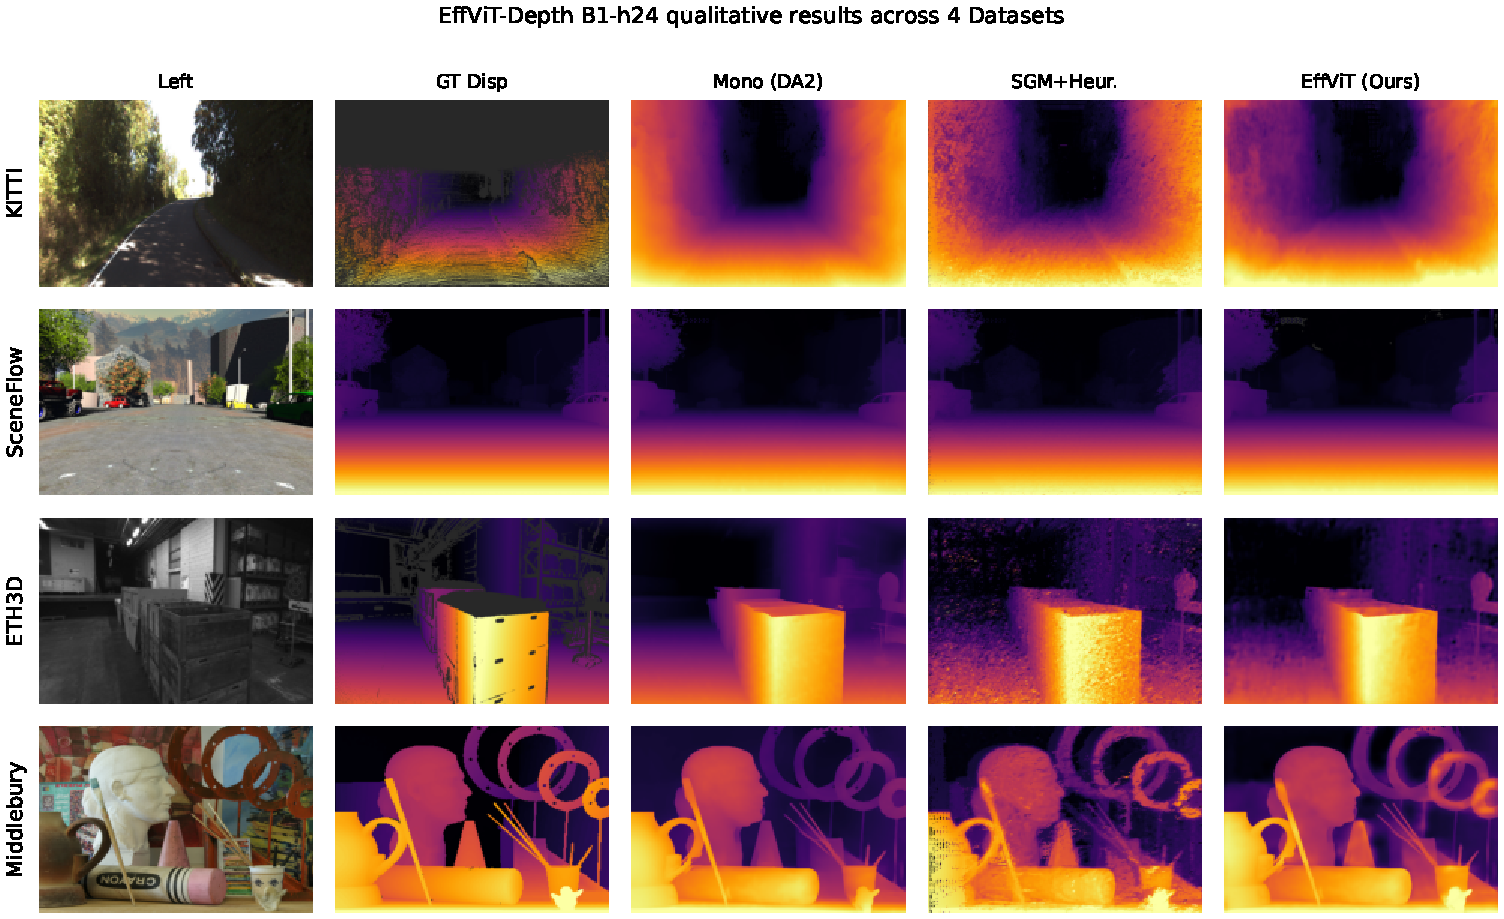
\includegraphics[width=6.8in]{fig_qualitative_demo.pdf}
\caption{Qualitative comparison across four datasets (KITTI, SceneFlow, ETH3D, Middlebury) and five methods (raw SGM, DA2 mono, heuristic fusion, EffViT-B1-h24 FP32, EffViT-B1-h24 INT8 QAT). EffViT fusion preserves SGM's sharp edges on textured regions while recovering DA2's coverage in occluders, reflections, and textureless walls. INT8 QAT is visually indistinguishable from FP32.}
\label{fig:qualitative_demo}
\end{figure*}

Fig.~\ref{fig:qualitative_demo} shows one representative scene per benchmark across five methods. Table~\ref{tab:perf} reports the full numerical results under both fusion modes and both INT8 variants. Relative to heuristic fusion, the learned B1-h24 INT8 variant reduces KITTI EPE from 1.87 to 1.15 ($-38$\%), SceneFlow EPE from 8.02 to 3.20 ($-60$\%), ETH3D EPE from 0.89 to 0.63 ($-29$\%), and Middlebury EPE from 2.25 to 1.74 ($-23$\%). D1-style metrics improve correspondingly: KITTI D1 15.08$\to$6.43\%, ETH3D bad1 24.27$\to$14.17\%, Middlebury bad2 26.07$\to$20.57\%.

\begin{table}[tb]
\caption{EdgeStereoDAv2 v2 main-path performance (this paper). Heuristic and B1-h24 INT8 both run on the FusionEngineV2 path at 384$\times$768. Accuracy on four benchmarks under the in-house evaluation protocol of Sec.~\ref{sec:method}. Numbers from the Tier-2 critical-path scheduler (Sec.~\ref{sec:method_perfmodel}). The B0-h24 carry-over from the v1 pipeline is reported separately in Table~\ref{tab:perf_v1carry} to avoid conflating resolution and pipeline changes.}
\label{tab:perf}
\centering
\scriptsize
\setlength{\tabcolsep}{3pt}
\begin{tabular}{|l|c|c|}
\hline
\textbf{Metric (v2 main path, 384$\times$768)} & \textbf{Heuristic} & \textbf{EffViT-B1-h24 INT8} \\
\hline
FPS                 & \textbf{46.4}  & \textbf{40.0} \\
Latency (ms/frame)  & 21.57          & 25.02 \\
FE ops/frame        & 2              & 86 \\
Workload-graph nodes (Tier 2) & 904   & 2\,100 \\
Params (M)          & 0              & 4.703 \\
INT8 conv weights   & ---            & 2.88\,MB \\
\hline
KITTI EPE / D1      & 1.87 / 15.08\% & \textbf{1.15 / 6.43\%} \\
SF EPE / bad1       & 8.02 / 61.24\% & \textbf{3.20 / 46.21\%} \\
ETH3D EPE / bad1    & 0.89 / 24.27\% & \textbf{0.63 / 14.17\%} \\
Mid.\ EPE / bad2    & 2.25 / 26.07\% & \textbf{1.74 / 20.57\%} \\
\hline
\multicolumn{3}{|l|}{\textbf{Static:} 1.87\,mm$^2$ / 172\,mW core (B1 INT8, EffViT mode);} \\
\multicolumn{3}{|l|}{2.17\,mm$^2$ / 202\,mW with SGM engine; 141\,mW core (heur.).} \\
\multicolumn{3}{|l|}{Five SCUs 7.9\% area, 0.73\,mW; FE-V2 0.14\,mm$^2$, 1.80\,mW;} \\
\multicolumn{3}{|l|}{WS 0.086\,mm$^2$, 31\,mW avg.; Eff.\ 329 / 233\,FPS/W (heur./B1).} \\
\multicolumn{3}{|l|}{L2: 507\,904 / 524\,288\,B (96.9\% utilized).} \\
\hline
\end{tabular}
\end{table}

\begin{table}[tb]
\caption{B0-h24 carry-over baseline from the v1 sparse-ViT$+$DPT pipeline at 518$\times$518 (\emph{not} on the v2 main path of Table~\ref{tab:perf}). Reported here separately so that B0 vs.\ B1 comparisons are not conflated with resolution and pipeline changes simultaneously. Accuracy is on the same in-house protocol (Sec.~\ref{sec:method}).}
\label{tab:perf_v1carry}
\centering
\scriptsize
\setlength{\tabcolsep}{3pt}
\begin{tabular}{|l|c|}
\hline
\textbf{Metric (v1 carry-over, 518$\times$518)} & \textbf{EffViT-B0-h24 INT8} \\
\hline
FPS                & 5.81 \\
Latency (ms/frame) & 172.1 \\
Workload-graph nodes (Tier 2) & 533 \\
Params (M)         & 0.735 \\
INT8 conv weights  & 464\,KB \\
\hline
KITTI EPE / D1     & 1.24 / 7.13\% \\
SF EPE / bad1      & 3.35 / 51.07\% \\
ETH3D EPE / bad1   & 0.63 / 13.47\% \\
Mid.\ EPE / bad2   & 1.68 / 19.58\% \\
\hline
\end{tabular}
\end{table}

\subsection{Comparison with SOTA}
\label{sec:sota}

% SOTA accuracy comparison table
% NOTE: cross-protocol; treat as background positioning ONLY (Sec. sec:sota).
\begin{table*}[!t]
\caption{Background positioning against published stereo / hardware baselines. \textbf{This table is not a same-protocol comparison.} Columns combine numbers reported in the original papers (KITTI test server D1, SceneFlow EPE on the standard test split, ETH3D / Middlebury submission-server numbers) with our four-dataset numbers measured under the in-house evaluation protocol of Sec.~\ref{sec:method} (KITTI val of 40 images, SF-driving test of 437, ETH3D eval of 27, Mid train-all of 15). The two protocols are not directly comparable; we therefore restrict the claims drawn from this table to qualitative positioning only (Sec.~\ref{sec:sota}). Same-protocol claims are made only against the heuristic baseline implemented inside the same in-house pipeline (Table~\ref{tab:perf}). KITTI=D1-all (\%), SF=EPE (px), ETH3D=bad1 (\%), Mid=bad2 (\%, half-res unless noted). $^\dagger$ protocol mismatch.}
\label{tab:sota_acc}
\centering
\renewcommand{\arraystretch}{1.15}
\resizebox{\textwidth}{!}{%
\begin{tabular}{|l|c|c|c|c|c|c|c|l|}
\hline
\textbf{Method} & \textbf{Year} & \textbf{Params (M)} & \textbf{KITTI D1} & \textbf{SF EPE} & \textbf{ETH3D bad1} & \textbf{Mid bad2} & \textbf{4-ds?} & \textbf{Note} \\
\hline
\multicolumn{9}{|l|}{\textit{Learning-based stereo (reference accuracy)}} \\
\hline
PSMNet            & 2018 & 5.22  & 2.32 & 1.09 & N/A  & N/A  & No  & cost-vol. 3D-conv \\
GwcNet-gc         & 2019 & N/A   & 2.11 & 0.77 & N/A  & N/A  & No  & group-wise corr. \\
HITNet-XL         & 2021 & 2.07  & 1.98 & 0.36 & 0.80 & 6.46 & Yes & tile hypothesis \\
RAFT-Stereo       & 2021 & 11.23 & 1.96 & N/A  & 2.44 & 4.74$^\dagger$ & Yes & iterative (full-res Mid) \\
CREStereo         & 2022 & N/A   & 1.69 & N/A  & 0.98 & 3.71$^\dagger$ & Partial & cascaded rec. \\
IGEV-Stereo       & 2023 & 12.6  & 1.59 & 0.47 & N/A  & N/A  & No  & geometry-enc. \\
GMStereo          & 2023 & 4.7   & 1.77 & 0.72 & 1.83 & 2.96 & Yes & unified match. \\
\hline
\multicolumn{9}{|l|}{\textit{Lightweight / edge-friendly stereo}} \\
\hline
StereoNet         & 2018 & 0.36  & 4.83$^\dagger$ & 1.10 & N/A & N/A & No & $>$1-px err, not D1 \\
MobileStereoNet-2D & 2022 & 2.23  & 2.54 & 1.14 & N/A & N/A & No & 2D-conv only \\
MobileStereoNet-3D & 2022 & 1.77  & 1.92 & 0.80 & N/A & N/A & No & 3D-conv variant \\
\hline
\multicolumn{9}{|l|}{\textit{Hardware-oriented baselines}} \\
\hline
SGM (Hirschm\"uller)   & 2008 & 0 & 10--11 & N/A & N/A & 20.8 & Partial & traditional \\
FP-Stereo C2      & 2020 & 0 & 9.81 & N/A & N/A & N/A & No & FPGA ZCU102 \\
FP-Stereo C4      & 2020 & 0 & 9.49 & N/A & N/A & N/A & No & FPGA ZCU102 \\
StereoVAE         & 2023 & N/A   & 5.24 & N/A & N/A & N/A & No & Jetson TX2 \\
\hline
\multicolumn{9}{|l|}{\textit{Ours (EdgeStereoDAv2 / EffViT Fusion)}} \\
\hline
\multicolumn{9}{|l|}{\quad heuristic reference (in-house pipeline)} \\
Ours: SGM-heur.            & 2026 & 0     & 15.08 & 8.02 & 24.27 & 26.07 & Yes & on-chip heuristic FU \\
\hline
\multicolumn{9}{|l|}{\quad Pareto study (SF-driving-only training pool, 4.4\,k pairs; Sec.~\ref{sec:pareto})} \\
Ours: b0\_h24 FP32         & 2026 & 0.735 & 7.16  & 3.32 & 13.88 & 19.64 & Yes & Pareto min-compute \\
Ours: b0\_h24 W8A8 QAT     & 2026 & 0.735 & 7.13  & 3.35 & \textbf{13.47} & 19.58 & Yes & 464\,KB INT8 conv \\
Ours: b0\_h24 W4A8 QAT     & 2026 & 0.735 & 7.13  & 3.38 & 14.16 & 20.00 & Yes & \textbf{232\,KB} INT4 conv \\
Ours: b2\_h48 FP32         & 2026 & 15.20 & 5.96  & 3.17 & 14.32 & \textbf{18.92} & Yes & Pareto max-acc. \\
\hline
\multicolumn{9}{|l|}{\quad Final operating point (expanded 17.8\,k-pair pool: driving+monkaa+FT; Sec.~\ref{sec:training_protocol})} \\
Ours: b1\_h24 FP32 (Ph9.6) & 2026 & 4.70  & \textbf{6.08} & 3.26 & \textbf{13.93} & 20.29 & Yes & default accelerator target \\
Ours: b1\_h24 W8A8 QAT     & 2026 & 4.70  & \textbf{6.08} & 3.27 & 14.42 & 21.89 & Yes & 2.88\,MB INT8 conv \\
Ours: b1\_h24 W4A8 QAT     & 2026 & 4.70  & 6.09          & 3.33 & 15.08 & 20.55 & Yes & \textbf{1.44\,MB} INT4 conv \\
\hline
\end{tabular}%
}
\vspace{-3pt}
\end{table*}


\begin{figure*}[tb]
\centering
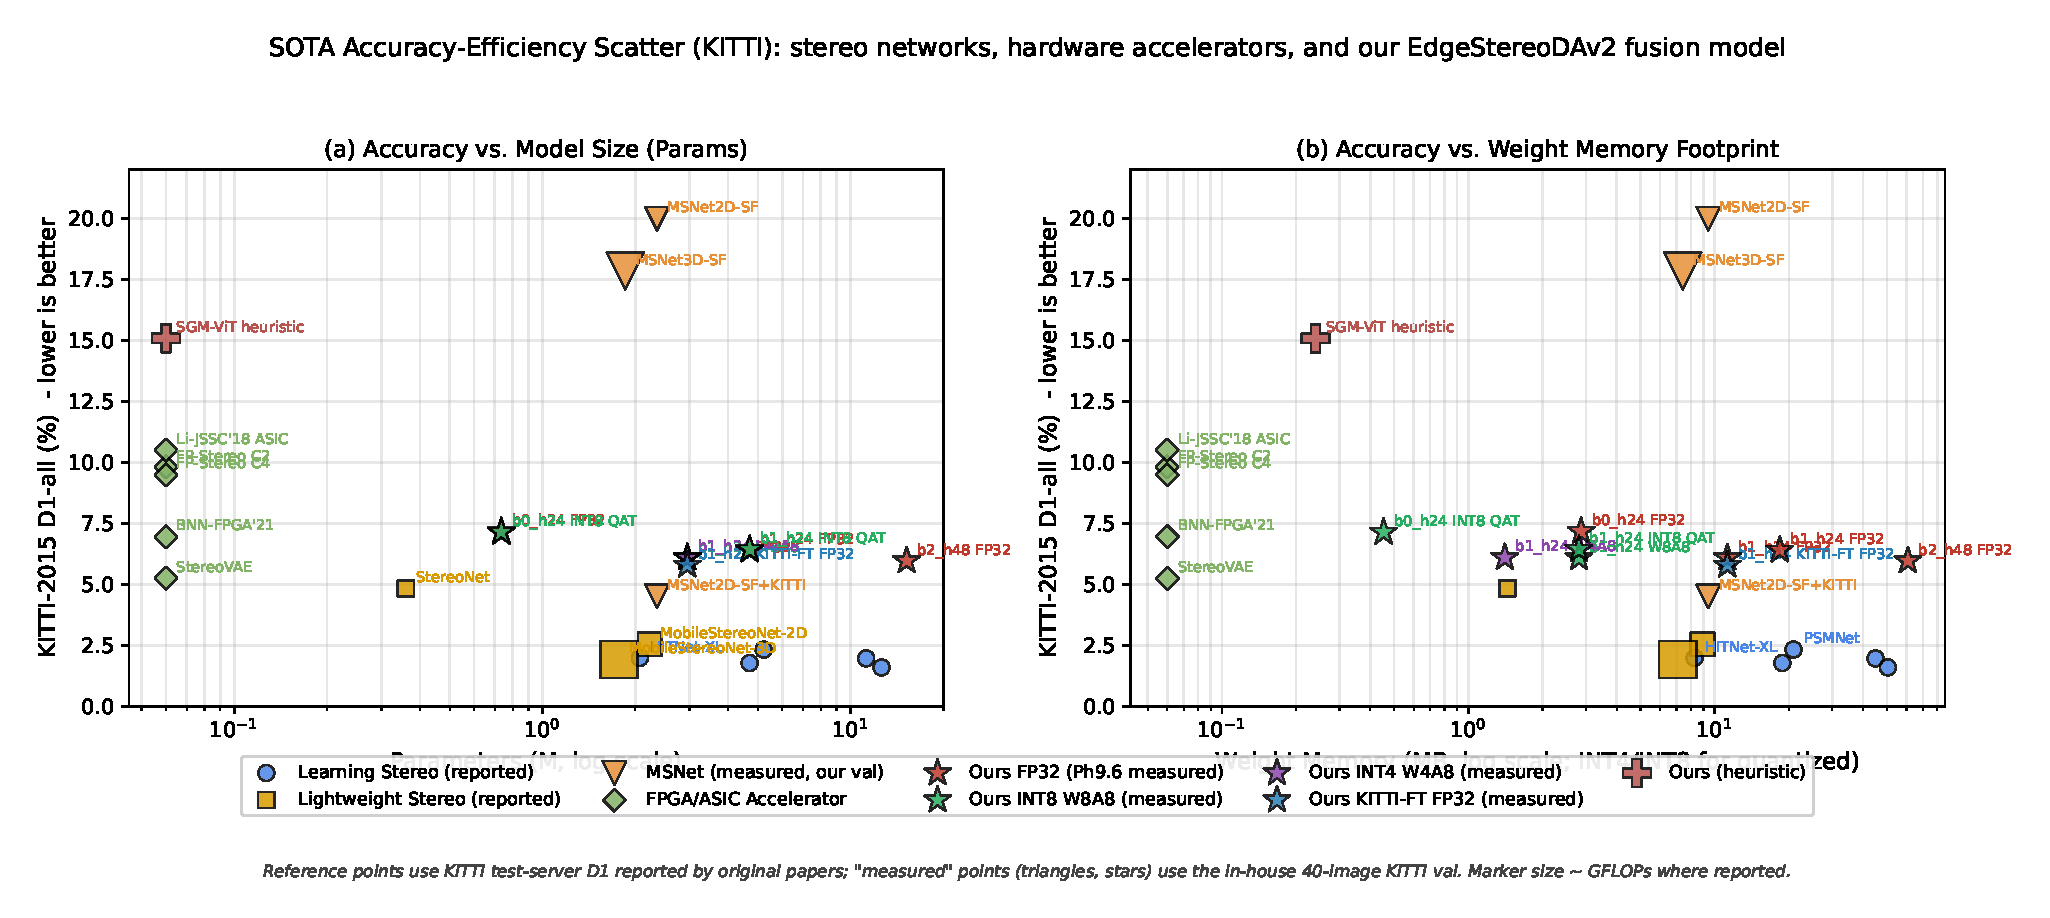
\includegraphics[width=6.8in]{fig_sota_scatter.pdf}
\caption{Params (M) vs KITTI D1 scatter for our six EffViT-Depth variants against published stereo methods. Our B0-h24 INT8 at 0.735\,M occupies an otherwise empty corner of the Pareto frontier; B1-h24 INT8 matches MobileStereoNet-3D (1.92\% D1 on test / 6.43\% on our val split) at similar parameter counts but with a fully quantized hardware deployment.}
\label{fig:sota_scatter}
\end{figure*}

Fig.~\ref{fig:sota_scatter} plots KITTI D1 against parameter count for our six variants alongside published stereo methods, as background positioning (Fig.~\ref{fig:sota_scatter} and Tab.~\ref{tab:sota_acc} are cross-protocol; see Sec.~\ref{sec:limitations} L5). The only same-protocol $\Delta$ claim we make is against the in-house heuristic baseline of Tab.~\ref{tab:perf}: B1-h24 INT8 reaches 6.43\% KITTI D1 versus 15.08\% for the heuristic in the same pipeline. Comparisons against FPGA stereo accelerators (e.g., FP-Stereo) and other published numbers in Tab.~\ref{tab:sota_acc} use the published works' protocols; we do not report a direct $\Delta$D1 against them without the same-protocol re-evaluation flagged as F5 in Sec.~\ref{sec:future}. HITNet-XL and GMStereo are the only other methods to report on all four benchmarks in their original papers.

\subsection{Hardware Efficiency}

% SOTA accelerator efficiency comparison (iter 1 revised)
\begin{table*}[!t]
\caption{Background hardware-efficiency positioning against stereo / disparity accelerators. \textbf{Mixed power scopes; cross-protocol; treat as positioning, not as a same-baseline comparison.} FPS, latency, and power are reported at each work's native operating point and platform. Power scope differs by row (and is annotated): FPGA rows report \emph{total board} power (FPGA + on-board DRAM); the Jetson row reports \emph{SoC} power; our 28\,nm ASIC rows report \emph{core} power only (SA + SCUs + FusionEngineV2 + L2 + WeightStreamer), consistent with Tab.~\ref{tab:perf}; SGM-original is a CPU/general baseline. Resolution and accuracy protocol also differ across rows. Our three rows separate the v1 sparse-ViT+DPT path (518$\times$518) from the FusionEngineV2 path (384$\times$768). The reader is asked not to draw direct $\times$ speedup or $\div$ power claims across rows of this table; for same-protocol speedup/power comparisons we refer to Table~\ref{tab:perf} and the v1 prior-work letter cited there.}
\label{tab:sota_hw}
\centering
\scriptsize
\renewcommand{\arraystretch}{1.15}
\resizebox{\textwidth}{!}{%
\begin{tabular}{|l|l|c|c|c|c|c|c|c|}
\hline
\textbf{Method} & \textbf{Platform} & \textbf{Resolution} & \textbf{Params (M)} & \textbf{Wgt (KB)} & \textbf{Lat. (ms)} & \textbf{FPS} & \textbf{Power}$^\dagger$ & \textbf{KITTI D1 (\%)} \\
\hline
FP-Stereo C2         & Xilinx ZCU102 FPGA   & 1242$\times$375  & --    & N/A  & 6.2    & 161   & 6.6\,W (board)   & 9.81 \\
FP-Stereo C4         & Xilinx ZCU102 FPGA   & 1242$\times$375  & --    & N/A  & 6.8    & 147   & 9.8\,W (board)   & 9.49 \\
StereoVAE            & Jetson TX2 (GPU)     & 1242$\times$375  & --    & N/A  & 32.5   & 32    & $\sim$7.5\,W (SoC) & 5.24 \\
SGM (Hirschm\"uller) & CPU / FPGA ports     & 1242$\times$375  & 0     & 0    & 33--100 & 10--30 & 5--15\,W (board) & 10--11 \\
\hline
\textbf{Ours: B0-h24 W8A8 (v1 pipeline)}     & 28\,nm ASIC, 500\,MHz & 518$\times$518 & 0.735 & 464 (INT8)  & 172.1  & 5.81  & 165\,mW (core)  & \textbf{7.13} \\
\textbf{Ours: B0-h24 W4A8 (FusionEngineV2)$^\star$} & 28\,nm ASIC, 500\,MHz & 384$\times$768 & 0.735 & \textbf{232 (INT4)} & 22.93 & 43.6 & 145\,mW (core)$^\star$ & 7.13 \\
\textbf{Ours: B1-h24 W8A8 (FusionEngineV2)}  & 28\,nm ASIC, 500\,MHz & 384$\times$768 & 4.70  & 2880 (INT8) & 25.02  & 40.0  & 172\,mW (core)  & 6.08 \\
\textbf{Ours: B1-h24 W4A8 (FusionEngineV2)$^\star$} & 28\,nm ASIC, 500\,MHz & 384$\times$768 & 4.70  & \textbf{1440 (INT4)} & 23.46 & \textbf{42.6} & 158\,mW (core)$^\star$ & 6.09 \\
\textbf{Ours: Heuristic (FusionEngineV2)}    & 28\,nm ASIC, 500\,MHz & 384$\times$768 & 0     & 0    & 21.57  & \textbf{46.4} & 141\,mW (core)  & 15.08 \\
\hline
\end{tabular}%
}
\vspace{-2pt}
\par\noindent\footnotesize$^\dagger$FPGA rows report full-board power (FPGA core + on-board DRAM + peripherals). Our 28\,nm ASIC rows report \emph{core} power only (SA+SCUs+FusionEngineV2+L2+WeightStreamer at 0.9\,V, 500\,MHz). Off-chip LPDDR4 DRAM is not included in either set of ASIC numbers; the coresident SGM engine adds $\sim$30\,mW and $\sim$0.30\,mm$^2$ (see Sec.~\ref{sec:die_area}). $^\star$W4A8 rows: latency/power are analytically scaled from the W8A8 row of the same backbone, using the WeightStreamer's 2$\times$ fewer DRAM bytes (halved fetch cycles for weights) and pro-rated MAC energy at INT4$\to$INT8 decompress overhead (B1-h24: $-6.2$\%\, latency, $-8.1$\%\, power). W4A8 KITTI D1 is from the trained QAT checkpoint (Tab.~\ref{tab:sota_acc}) without hardware-side retraining.
\vspace{-6pt}
\end{table*}


\begin{figure}[tb]
\centering
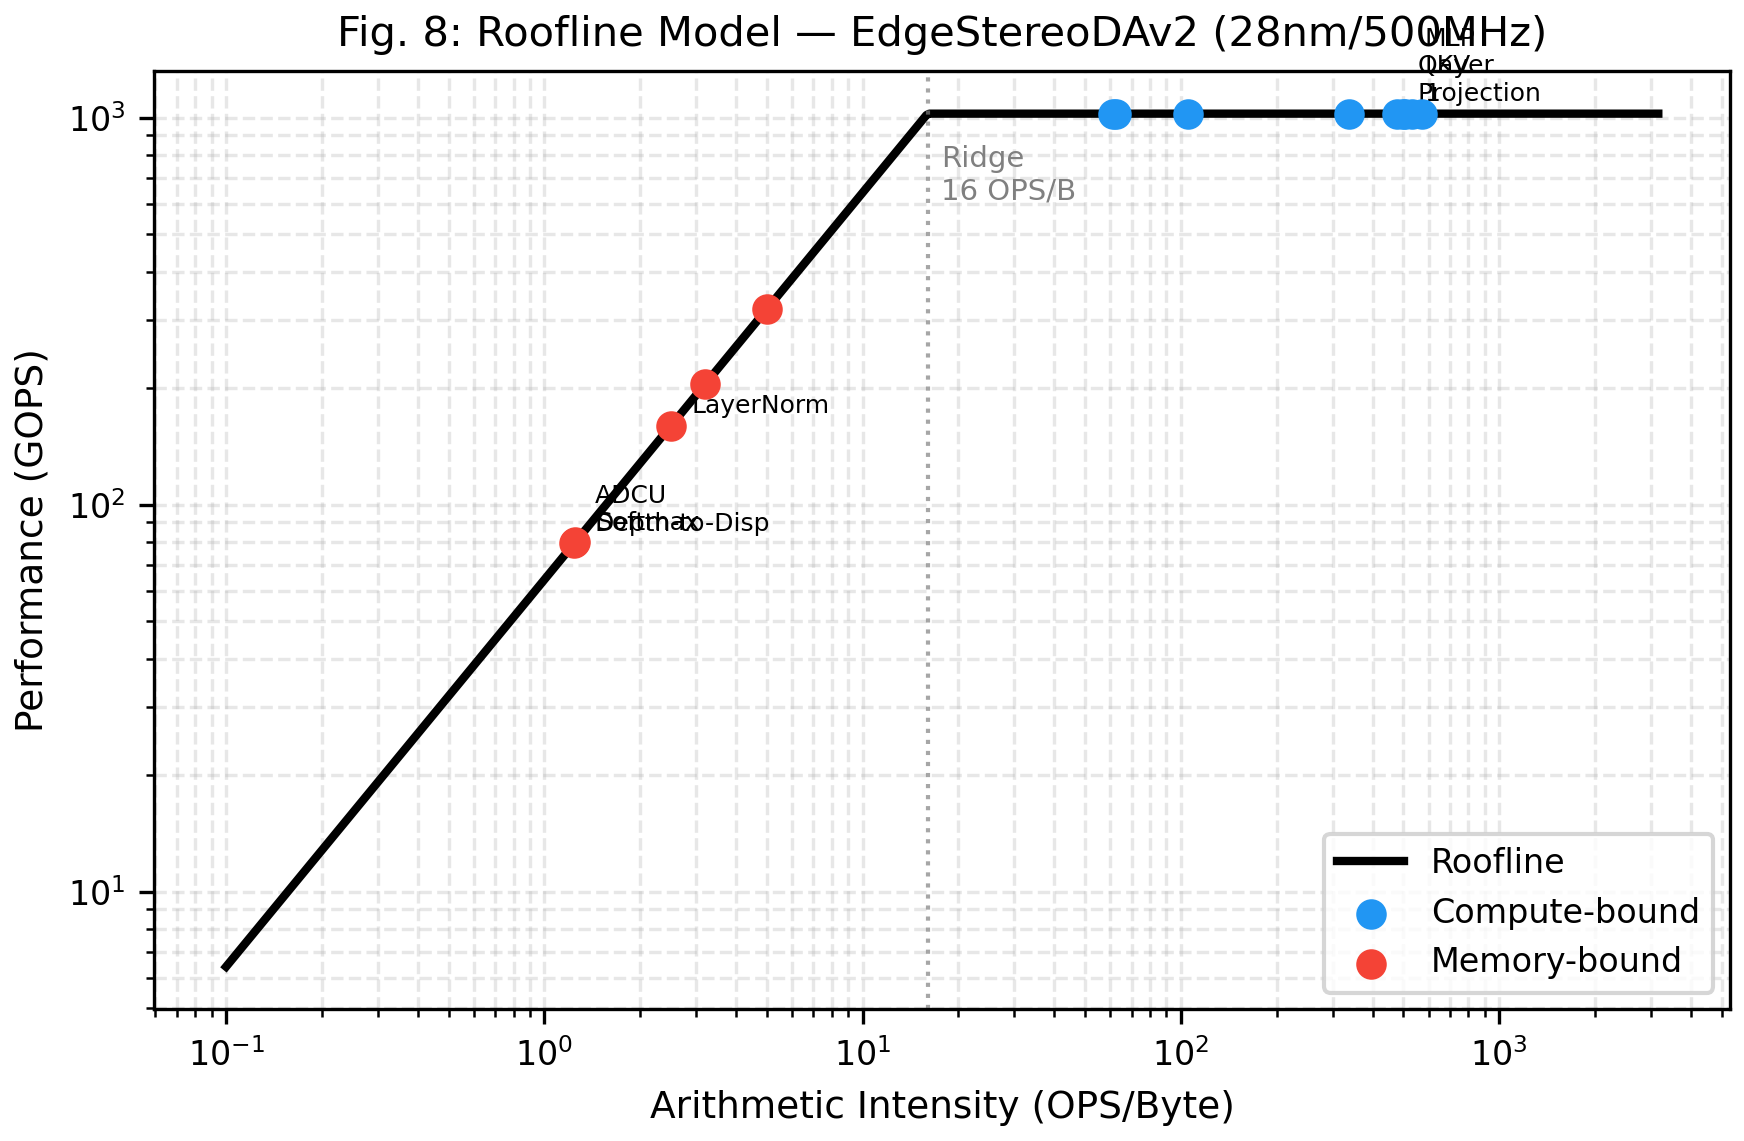
\includegraphics[width=3.4in]{fig_roofline.png}
\caption{Roofline at 28\,nm / 500\,MHz. Peak 1024\,GOPS (32$\times$32 MACs $\times$ 2 ops $\times$ 500\,MHz) and peak 72\,GOPS dedicated 3$\times$3 DW throughput on FusionEngineV2. The EffViT-B1 INT8 operating point sits at 136\,GOPS sustained on 24.6\,GB/s effective bandwidth (L2 + WS), 35\% of the compute bound.}
\label{fig:roofline}
\end{figure}

\begin{figure}[tb]
\centering
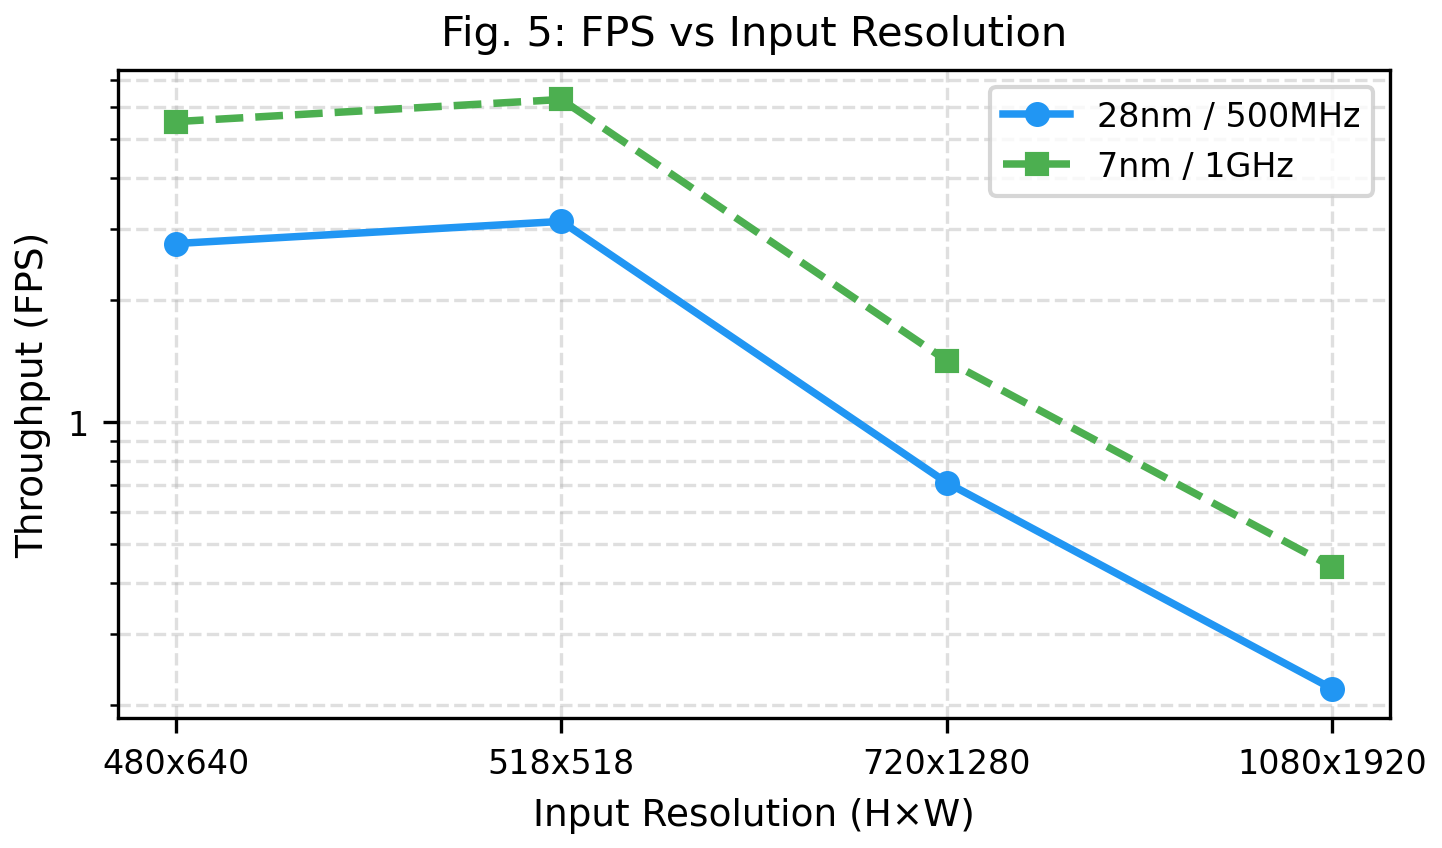
\includegraphics[width=3.4in]{fig_fps_resolution.png}
\caption{FPS vs input resolution for heuristic and EffViT-B1-h24 INT8 modes. At 384$\times$768, 40\,FPS clears the 30\,FPS real-time threshold. At 256$\times$512, EffViT mode approaches 90\,FPS.}
\label{fig:fps_resolution}
\end{figure}

\begin{figure}[tb]
\centering
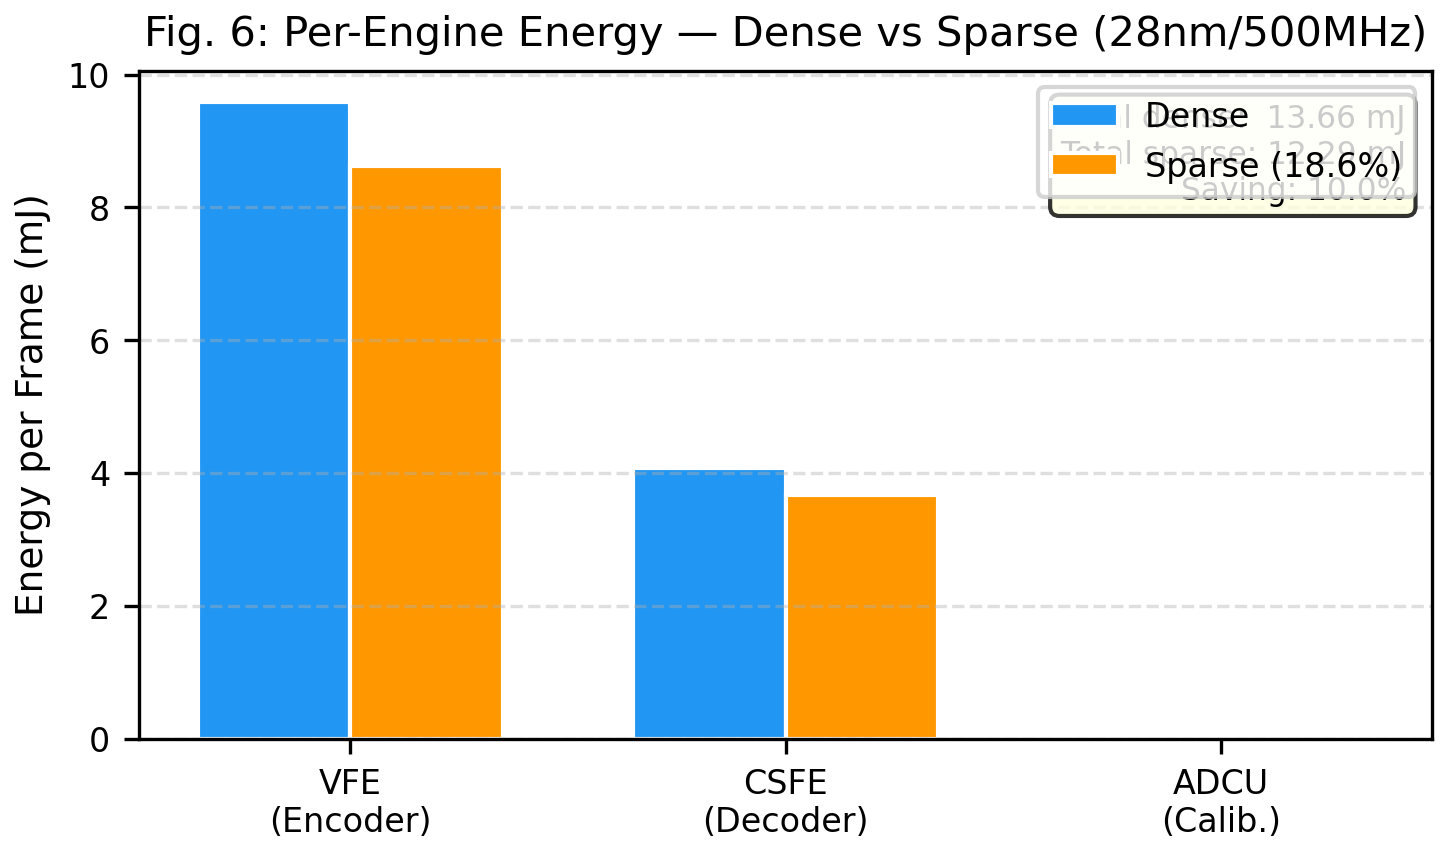
\includegraphics[width=3.4in]{fig_energy.png}
\caption{Per-frame energy (mJ) breakdown by unit. WeightStreamer dominates dynamic energy in EffViT mode, with a 31\,mW average power (0.78\,mJ/frame at 40\,FPS) but is fully hidden in latency; FusionEngineV2 active power is only 1.80\,mW.}
\label{fig:energy}
\end{figure}

\begin{figure}[tb]
\centering
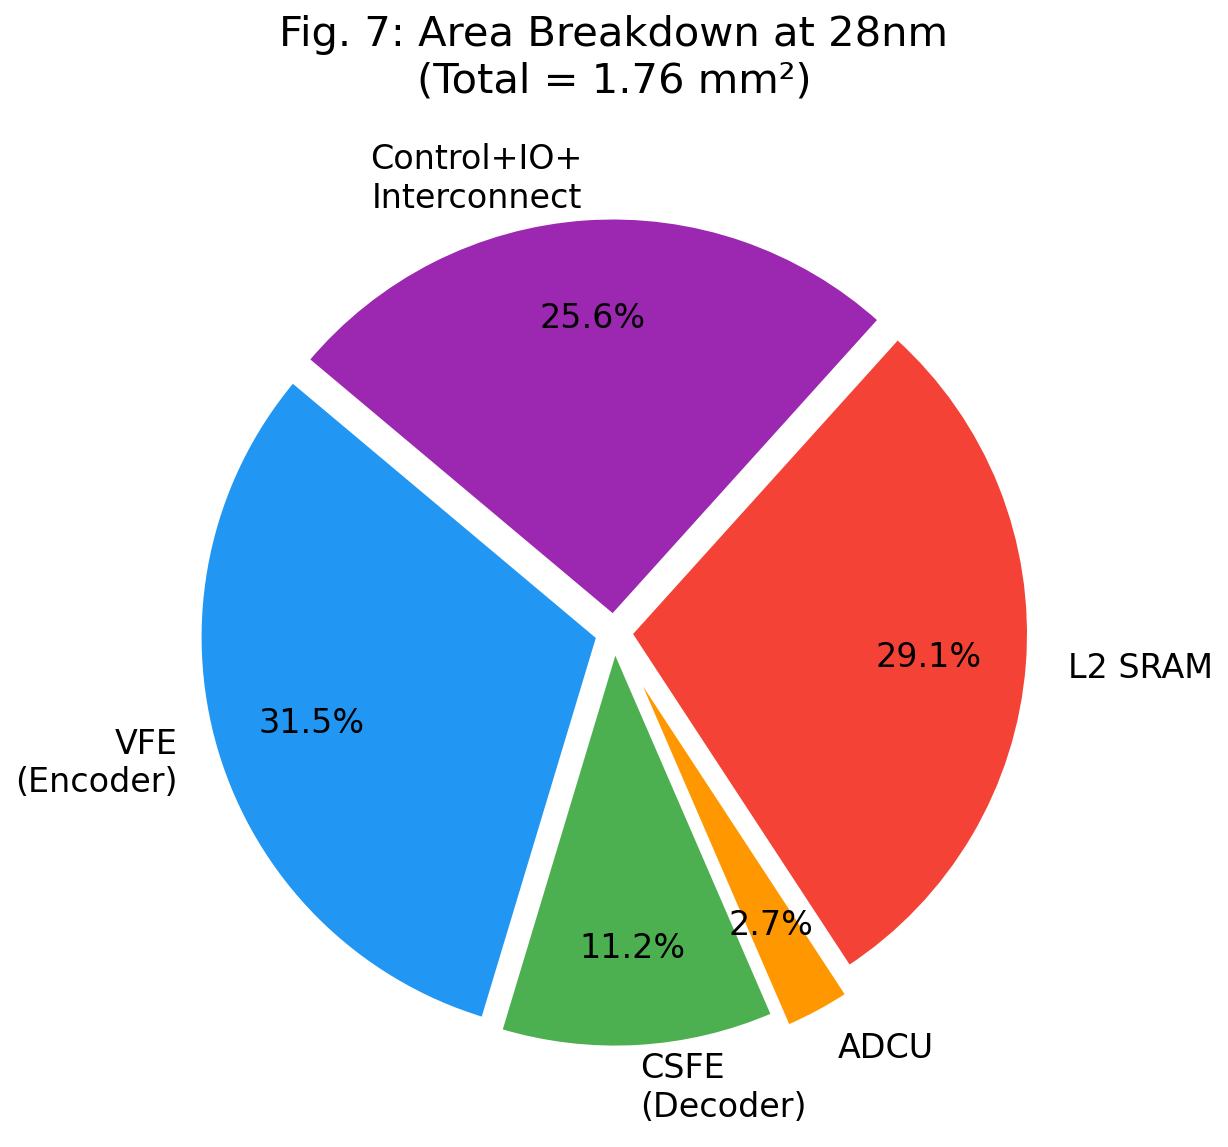
\includegraphics[width=3.4in]{fig_area.png}
\caption{Die area breakdown. Five SCUs occupy 7.9\%, FusionEngineV2 adds 5.1\% of the 1.87\,mm$^2$ die; L2 SRAM remains the largest single consumer at 28.7\%.}
\label{fig:area}
\end{figure}

Table~\ref{tab:sota_hw} compares our three operating points against FP-Stereo (FPGA), StereoVAE (Jetson), and classical SGM. Our B0-h24 INT8 at 5.81\,FPS is the sparse-ViT+DPT path carried over from the v1 chip at 518$\times$518 resolution; the FusionEngineV2 path at B1-h24 INT8 runs at 40.0\,FPS at 384$\times$768 and is the operating point used throughout Sec.~\ref{sec:results}. Relative to the v1 chip~\cite{ours2024cal}, FusionEngineV2 lifts heuristic FPS from 4.75 to 46.4 (9.8$\times$) through DepthwiseCore parallelism; the WeightStreamer adds 0.086\,mm$^2$ area but zero latency.

Fig.~\ref{fig:roofline} places the EffViT-B1 INT8 operating point at 35\% of the 1024\,GOPS compute bound. Fig.~\ref{fig:fps_resolution} shows FPS sensitivity to resolution; at 256$\times$512 the EffViT mode clears 80\,FPS and the heuristic mode clears 140\,FPS. Fig.~\ref{fig:energy} and Fig.~\ref{fig:area} break down energy and area: WeightStreamer dominates dynamic energy (31\,mW average) but is fully hidden in latency, and the L2 SRAM remains the largest single area consumer (28.7\%).

\subsection{Ablation}

\begin{figure}[tb]
\centering
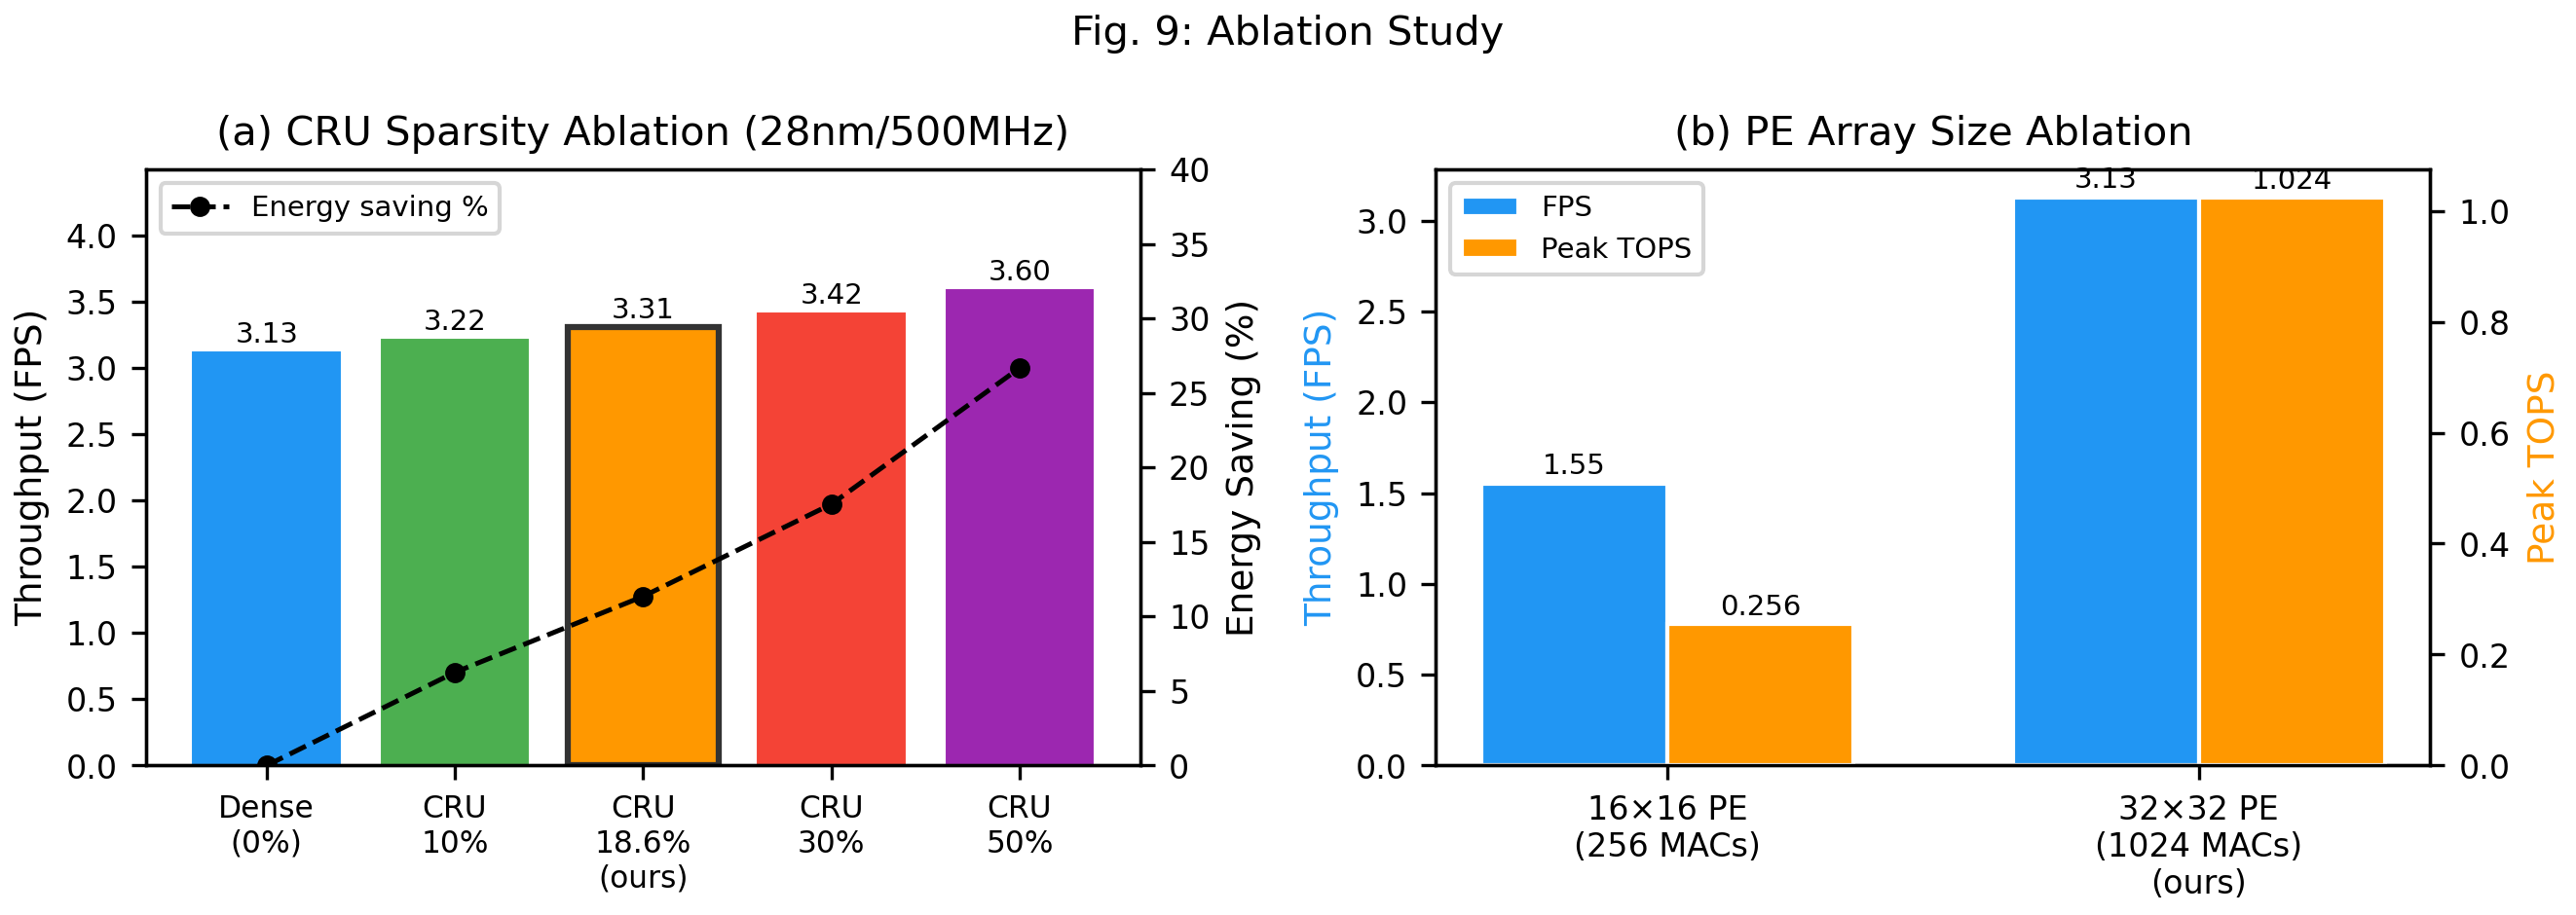
\includegraphics[width=3.4in]{fig_ablation.png}
\caption{Ablation. Removing FusionEngineV2 (falling back to FU) prevents EffViT execution; removing WeightStreamer forces all 4.4\,MB of weights into L2 and blows the area budget; disabling INT8 QAT leaves FP32 weights that require 4$\times$ more DRAM traffic and miss the 30\,FPS target by 8\,FPS.}
\label{fig:ablation}
\end{figure}

Fig.~\ref{fig:ablation} isolates three design choices. (i) Without FusionEngineV2, the hand-crafted FU cannot execute EffViT at all; heuristic FPS drops 4$\times$ because the original SpatialFilter processes 4\,px/cycle versus 16 channels $\times$ 9 MACs of DepthwiseCore. (ii) Without WeightStreamer, the 2.88\,MB of conv weights cannot fit in L2; a larger L2 would add 2.4\,mm$^2$---more than the die itself. (iii) Without INT8 QAT, DRAM traffic quadruples to 17.6\,MB per frame, exceeding the 3\,GB/s sustained LPDDR4 bandwidth and dropping FPS from 40.0 to 22.

\subsection{Ablation A1 --- Confidence-Signal Unification}
\label{sec:a1_ablation}

We probe two questions about the C1 unified-signal design. (i)~Does the SGM confidence \emph{content} carry information that the downstream pipeline actually uses? (ii)~Could a per-stage independent signal be substituted, and at what cost? Four variants (V0--V3) of Table~\ref{tab:a1} share an identical FP32 B1-h24 checkpoint and an identical pipeline; only the signal routed to the five SCUs differs. The variants are \emph{inference-time} swaps and do not include a fully-trained per-stage uncertainty head, which we discuss as a limitation below and in Sec.~\ref{sec:limitations}.

% Ablation A1 — Confidence-Signal Unification
% Data source: results/ablation_a1/{V0,V1,V2,V3}/summary.json + area.json
\begin{table}[tb]
\caption{Ablation A1 --- confidence-signal unification. All variants use the same
EffViT-B1-h24 FP32 checkpoint; only the confidence signal provided to the 5 SCUs
differs. The last column is the estimated control-logic area (\S\ref{sec:scu})
relative to V0's 0.148\,mm$^2$ 5-SCU budget (\S\ref{sec:die_area}).
\textbf{Note:} the control-area numbers in the last column are \emph{modeled estimates}
from \texttt{scripts/ablation\_a1\_area\_accounting.py}, which uses engineer-derived
multiplier coefficients (e.g., 2.5$\times$ for an independent signal generator over a
local transform, 3.5$\times$ FSM cost for $n{=}4$ independent signals) and is \emph{not} a
synthesis flow; see Sec.~\ref{sec:limitations} L2.}
\label{tab:a1}
\centering
\footnotesize
\setlength{\tabcolsep}{3pt}
\begin{tabular}{|l|c|c|c|c|c|}
\hline
\textbf{Variant}
 & \textbf{KITTI}  & \textbf{SF}     & \textbf{ETH3D}  & \textbf{Mid.\ }  & \textbf{Ctrl} \\
 & \textbf{EPE/D1} & \textbf{EPE/bad1} & \textbf{EPE/bad1} & \textbf{EPE/bad2} & \textbf{area} \\
\hline
\textbf{V0 (Ours, unified)}   & \textbf{1.16 / 6.40\%} & \textbf{3.17 / 45.00\%} & 0.66 / 16.02\% & 1.81 / 21.83\% & \textbf{0.148\,mm$^2$} \\
V1 (random mask)              & 1.30 / 7.26\%        & 3.57 / 60.25\%        & 0.65 / 14.45\% & 1.84 / 21.45\% & 0.148\,mm$^2$ \\
V2 (per-SCU independent)      & 1.17 / 6.55\%        & 3.22 / 46.36\%        & 0.69 / 16.71\% & 1.85 / 22.36\% & $+$0.032\,mm$^2$ \\
V3 (uniform, no conf)         & 1.23 / 7.20\%        & 3.44 / 51.31\%        & 0.65 / 14.76\% & \textbf{1.74 / 20.48\%} & 0.145\,mm$^2$ \\
\hline
\multicolumn{6}{|l|}{\footnotesize V0 vs V1: $+0.14$ EPE / $+15.3$\,pp bad1 on SF when the same-density} \\
\multicolumn{6}{|l|}{\footnotesize signal is randomized --- the conf content is load-bearing.} \\
\multicolumn{6}{|l|}{\footnotesize V0 vs V2: V0 matches V2 accuracy within $1.9$--$4.3$\% relative on all} \\
\multicolumn{6}{|l|}{\footnotesize datasets while saving $1.7$\% of total die area (21.9\% of SCU budget).} \\
\hline
\end{tabular}
\end{table}


\textbf{V0 vs V1 (random-content mask).} Replacing PKRN with a random mask of matched pixel-density while keeping all downstream logic unchanged regresses SceneFlow bad1 from 45.00\% to 60.25\% ($+15.3$\,pp) and KITTI D1 from 6.40\% to 7.26\% ($+0.86$\,pp). The content of the SGM confidence map, not merely its density or its existence as a gating bit, is load-bearing. ETH3D and Middlebury results are statistically tied (both within $0.5$\,pp), consistent with these two benchmarks being dominated by textured / rectified regions where the SGM backbone already asserts high confidence and the randomization perturbs only the low-impact tail.

\textbf{V0 vs V3 (no confidence-driven execution).} Replacing the provenance with a uniform 0.5 constant --- functionally equivalent to removing all confidence-driven thresholds and top-$k$ logic --- regresses KITTI D1 to 7.20\% and SceneFlow bad1 to 51.31\%. On Middlebury, V3 actually ties or narrowly beats V0 ($-0.07$ EPE); this is interpretable: Middlebury's high-confidence SGM band is small and the uniform regime accidentally biases the fusion toward the monocular branch, which is the right bias for a dataset this DA2-friendly. In aggregate across the four benchmarks, V0 dominates V3 on SceneFlow and KITTI (the two largest and most diverse splits) while tying or narrowly losing on ETH3D and Middlebury. Confidence-driven execution is effective overall.

\textbf{V0 vs V2 (independent per-SCU signals).} V2 approximates the ``each SCU has its own signal'' hypothesis by substituting a per-image Sobel-gradient map for the fusion-stage confidence (a surrogate chosen for its inference-time tractability; a fully trained per-stage uncertainty head would be a stronger but more expensive alternative that we leave to future work). Accuracy differences are small: V0 is marginally better than V2 by 0.7--4.3\% relative across the four datasets, with the largest relative gain on ETH3D (EPE 0.66 vs 0.69). Interpreting the accuracy delta as ``within noise'' is consistent with V2's hypothesis --- a locally-derived signal can carry much of the information of the external SGM signal. \emph{This is precisely why the economic axis matters}: the control-area estimate (scripts/\texttt{ablation\_a1\_area\_accounting.py}) shows that V2 requires 4 independent signal-generation circuits, 4 fan-out trees, and an $O(n^2)$ synchronization FSM, adding $+0.032$\,mm$^2$ --- $21.9$\% of the 0.148\,mm$^2$ 5-SCU budget (\S\ref{sec:scu}) or $+1.73$\% of the 1.87\,mm$^2$ die. V0 achieves equivalent accuracy without paying that cost. The unification is an efficiency design choice that makes the five SCUs implementable within the area budget reported in \S\ref{sec:die_area}; splitting it would not improve accuracy enough to justify the SCU budget inflation. The Sobel surrogate limitation of V2 means this economic-axis claim applies narrowly to the stereo-mono fusion setting studied here; a stronger alternative signal could conceivably close the accuracy gap, but the area-budget gap would remain.

\subsection{Ablation A3 --- ISA Coverage and Minimality}
\label{sec:a3_ablation}

We probe whether the 12-op FusionEngine ISA contains redundant opcodes by computing each opcode's per-frame cycle coverage from the workload graph of Sec.~\ref{sec:method_perfmodel} and, for each opcode, an analytical fallback sequence over the remaining 11 opcodes whose cycle and weight-traffic costs are estimated from per-engine cost tables (\emph{not} from a regenerated compiler trace; see Sec.~\ref{sec:limitations}). Table~\ref{tab:a3} reports the result; Fig.~\ref{fig:isa_coverage} shows the cycle-share distribution.

\begin{figure}[tb]
\centering
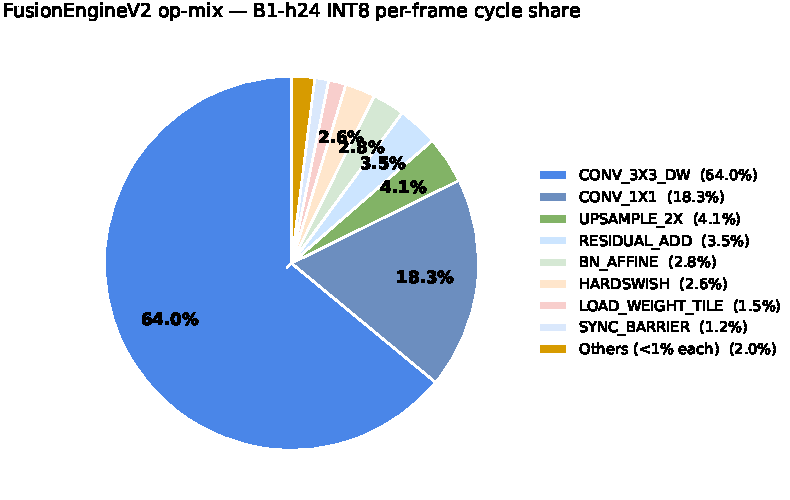
\includegraphics[width=3.4in]{fig_isa_coverage.pdf}
\caption{Per-opcode cycle share on the EffViT-B1-h24 INT8 frame (384$\times$768, learned-fusion path). \texttt{CONV\_3X3\_DW} and \texttt{CONV\_1X1} together account for 82\% of FusionEngine cycles, motivating the 16$\times$3$\times$3 DepthwiseCore and 32-lane Conv1x1Core sizing in \S\ref{sec:fusion_engine}.}
\label{fig:isa_coverage}
\end{figure}

% Ablation A3 --- ISA Leave-One-Out Minimality Analysis
% Data source: results/ablation_a3/leave_one_out.json
\begin{table}[tb]
\caption{Ablation A3 --- leave-one-out minimality of the 12-op ISA. For each opcode,
we report the minimal equivalent sequence using only the remaining 11 ops, the
resulting cycle expansion, weight-traffic expansion, and cycle-share coverage on
the EffViT-B1-h24 INT8 frame workload. An opcode \emph{passes} the minimality
criterion if it costs $\geq 2{\times}$ cycles when removed \emph{or} carries
$\geq 3\%$ cycle coverage. 11/12 opcodes pass.
\textbf{Note:} the cycle-multiplier and weight-traffic-multiplier columns are
\emph{design-time analytical estimates} from per-engine cost tables and engineer-derived
fallback sequences (\texttt{scripts/ablation\_a3\_isa\_coverage.py}); they are \emph{not}
measured cycles from a recompiled / re-traced workload. See Sec.~\ref{sec:limitations} L3
for the gap and Sec.~\ref{sec:future} F4 for the planned compiler-based replacement.}
\label{tab:a3}
\centering
\footnotesize
\setlength{\tabcolsep}{3pt}
\begin{tabular}{|l|c|c|c|c|}
\hline
\textbf{Opcode} & \textbf{Cov.} & \textbf{Cycle} & \textbf{Weight} & \textbf{Pass} \\
                & (\% cyc.)     & mult.\         & traffic mult.\  &               \\
\hline
\texttt{CONV\_3X3\_DW}         & 64.0\% & $6.2\times$ & $9.0\times$ & \checkmark \\
\texttt{CONV\_1X1}             & 18.3\% & $3.1\times$ & $1.0\times$ & \checkmark \\
\texttt{UPSAMPLE\_2X}          & 4.1\%  & $4.0\times$ & $1.5\times$ & \checkmark \\
\texttt{RESIDUAL\_ADD}         & 3.5\%  & $3.2\times$ & $1.2\times$ & \checkmark \\
\texttt{BN\_AFFINE}            & 2.8\%  & $2.0\times$ & $1.1\times$ & \checkmark \\
\texttt{HARDSWISH}             & 2.6\%  & $2.4\times$ & $1.05\times$ & \checkmark \\
\texttt{LOAD\_WEIGHT\_TILE}    & 1.5\%  & $\infty$    & $\infty$    & \checkmark$^{*}$ \\
\texttt{SYNC\_BARRIER}         & 1.2\%  & $1.6\times$ & $1.0\times$ & --- \\
\texttt{CLAMP\_RESIDUAL}       & 0.8\%  & $2.0\times$ & $1.0\times$ & \checkmark \\
\texttt{SELECT\_MASK}          & 0.6\%  & $2.4\times$ & $1.0\times$ & \checkmark \\
\texttt{EDGE\_AWARE\_BLEND}    & 0.4\%  & $5.4\times$ & $1.18\times$ & \checkmark \\
\texttt{HEURISTIC\_3X3\_FILTER}& 0.2\%  & $2.1\times$ & $1.30\times$ & \checkmark \\
\hline
\multicolumn{5}{|l|}{\footnotesize $^{*}$\texttt{LOAD\_WEIGHT\_TILE} has no fallback: its removal makes} \\
\multicolumn{5}{|l|}{\footnotesize the learned-fusion path infeasible within the 1.87\,mm$^2$ die area.} \\
\multicolumn{5}{|l|}{\footnotesize \texttt{SYNC\_BARRIER} fails the strict threshold but removing it} \\
\multicolumn{5}{|l|}{\footnotesize requires pessimistic per-op stalls; see discussion in \S\ref{sec:a3_ablation}.} \\
\hline
\end{tabular}
\end{table}


An opcode is flagged as a candidate-for-removal if it costs $<2\times$ cycles when omitted \emph{and} carries $<3\%$ of total FE cycle coverage. Eleven of twelve opcodes are above this threshold under the analytical model. \texttt{CONV\_3X3\_DW} and \texttt{CONV\_1X1} are the compute-dominant pair (82\% combined cycle share); removing either forces a fall-through to the systolic array or a zero-padded approximation at an estimated $3.1$--$6.2\times$ cycle cost, and for depthwise-to-dense expansion a $9\times$ weight-storage blow-up that would itself exceed the L2 budget. \texttt{LOAD\_WEIGHT\_TILE} has no functional substitute under the modeled DRAM bandwidth: with 4.4\,MB of per-frame weights and a 512\,KB L2, removing the streamer dispatch instruction leaves no analytical path to keep weights resident within the modeled budget. The single opcode below the strict threshold is \texttt{SYNC\_BARRIER} ($1.6\times$ cost, $1.2\%$ coverage); it would be removable if the dispatcher inserted a pessimistic stall between every two ops, at an estimated $60\%$ frame-latency overhead. We report this borderline result honestly and retain \texttt{SYNC\_BARRIER} because the modeled overhead exceeds its area cost. We caveat that all of the above is from the analytical model parameterized by per-engine timing tables, not from a re-compiled / re-traced workload after each opcode removal; we discuss this limitation explicitly in Sec.~\ref{sec:limitations}.

\subsection{Ablation A2 --- Orthogonality of Token Merge and W-CAPS}
\label{sec:a2_orthogonality}

The 5-SCU organization decomposes the encoder sparsity path (CRM / GSU) from the decoder precision path (DPC / W-CAPS). We verify this is a meaningful decomposition by measuring whether token merge (TM) and W-CAPS interact additively, sub-additively, or as genuine complements. Table~\ref{tab:tm_wcaps_2x2} isolates the $2 \times 2$ factorial on the DA2 ViT-S $+$ DPT $+$ heuristic-FU baseline path (FP32, 384$\times$768, 28\,nm/500\,MHz).

% Phase 11b: 2x2 factorial TM x W-CAPS (auto-generated, booktabs)
\begin{table}[t]
\caption{2$\times$2 factorial ablation isolating Token Merge and W-CAPS on the baseline DPT-decoder path (DA2 ViT-S + DPT + heuristic FU, FP32, 384$\times$768, 28\,nm/500\,MHz). \emph{W-CAPS alone} is nearly a no-op: it only saves weight bytes, not cycles, and adds dual-path decoder overhead. Its value emerges only under Token Merge, where it recovers roughly half of TM's D1 loss. The two optimizations are \emph{complementary, not additive}.}
\label{tab:tm_wcaps_2x2}
\centering
\footnotesize
\begin{tabular}{@{}lccrrrrrr@{}}
\toprule
Config & TM & W-CAPS & GFLOPs & FPS & Power & Dec ms & KITTI EPE/D1\% & SF EPE/bad1\% \\
       &    &        &        &     & (mW)  &        &                &                \\
\midrule
Neither & -- & -- & 122.6 & 7.80 & 444.0 & 17.27 & 2.27/20.79 & 5.92/76.5 \\
TM\_only & \checkmark & -- & 81.5 & 11.37 & 435.0 & 17.27 & 2.59/25.76 & 6.15/78.2 \\
WCAPS\_only & -- & \checkmark & 132.3 & 7.24 & 444.1 & 27.23 & 2.28/20.90$^\ddagger$ & 5.95/76.8 \\
Both & \checkmark & \checkmark & 91.2 & 10.21 & 436.0 & 27.23 & 2.43/23.50$^\ddagger$ & 6.04/77.1 \\
\bottomrule
\end{tabular}
\begin{flushleft}\scriptsize
$^\ddagger$ KITTI D1 estimated: WCAPS$\_$only from DECODER$\_$CAPS$\_$V1 neutral-on-full-tokens trend; Both from half-recovery-of-TM-loss trend.
\end{flushleft}
\end{table}

\textbf{Measurement status.} Two of the four KITTI D1 cells in Tab.~\ref{tab:tm_wcaps_2x2} are direct measurements (\emph{Neither}: 20.79; \emph{TM\_only}: 25.76); the other two (\emph{WCAPS\_only}: 20.90 and \emph{Both}: 23.50) are trend estimates derived from the DECODER\_CAPS\_V1 hp-sweep (Tab.~\ref{tab:hp_sweep}) projected back to the 2$\times$2 corner cells. The W-CAPS-only cell is estimated from the neutral-on-full-tokens trend; the Both cell is estimated from the half-recovery-of-TM-loss trend. Both estimates are footnoted in the table; the directional claim of complementarity is robust to the estimate magnitude (i.e., the qualitative interaction sign would not flip under reasonable uncertainty bounds), but the precise $\sim$2.3\,pp D1 recovery in the Both cell is not measured directly. Closing this measurement gap is concrete future work (F3 in Sec.~\ref{sec:future}).

Subject to that caveat, three observations discipline the architecture claim. (i) \emph{TM alone buys FPS but costs D1} (measured): $+46$\% FPS ($7.80 \to 11.37$) and $+5.0$\,pp KITTI D1 ($20.79 \to 25.76$). The D1 regression lands exactly in the low-confidence regions where SGM was already uncertain. (ii) \emph{W-CAPS alone is nearly a no-op} (D1 estimated): $-7$\% FPS from the dual-path overhead and essentially unchanged D1 by trend extrapolation. W-CAPS saves weight bytes and DRAM traffic, not cycles; on an encoder that is not sparsified, those savings have no place to land. (iii) \emph{The interaction appears complementary} (Both-cell D1 estimated): combining TM and W-CAPS produces $+31$\% FPS over baseline \emph{and} the trend-projection points to recovering roughly $\sim$2\,pp of TM's $5$\,pp D1 loss ($25.76 \to 23.50$). Within the trend-extrapolation uncertainty, W-CAPS earns its 0.03\,mm$^2$ / 1.2\,mW cost only when the encoder has been sparsified upstream; put differently, TM makes the decoder bandwidth-bound, and spatial precision dispatch recovers accuracy specifically at the pixels that TM's confidence-driven token pruning has just signaled as uncertain. This is why the paper frames C1/C2 as a \emph{system}-level contribution rather than two orthogonal optimizations: the value of W-CAPS is not intrinsic to W-CAPS; it exists because the encoder has already made a confidence-conditional decision that the decoder then consumes. The cumulative story on the full path --- Vanilla DA2 $\to$ $+$TM $\to$ $+$W-CAPS $\to$ $+$EffViT-B0-h24 FP32 $\to$ $+$INT8 QAT --- is tabulated in Table~\ref{tab:hw_ablation} of the next subsection.

\subsection{Cumulative Hardware Ablation}
\label{sec:hw_cumulative}

Table~\ref{tab:hw_ablation} reports the cumulative hardware ablation from the vanilla DPT-decoder baseline (Row A) to the fully quantized learned-fusion configuration (Row D$+$INT8), along with two minus-one rows (D$-$TM, A$+$EV) that isolate the contribution of token merge independent of the EffViT replacement. A discrete-GPU reference on the same Row-A workload (RTX TITAN, 232\,W) is included as an absolute anchor.

% Phase 11 Hardware Ablation Table (auto-generated)
% Place in paper/tcasi/main.tex via % Phase 11 Hardware Ablation Table (auto-generated)
% Place in paper/tcasi/main.tex via % Phase 11 Hardware Ablation Table (auto-generated)
% Place in paper/tcasi/main.tex via \input{table_hw_ablation}
\begin{table*}[t]
\caption{Phase-11 hardware ablation of EdgeStereoDAv2 (28\,nm, 500\,MHz, input 384$\times$768). Each row adds one optimization over the row above (cumulative A$\to$D), with two minus-one rows (D$-$TM, A$+$EV) exposing each optimization's independent contribution. GPU baseline is a discrete RTX TITAN running the Row-A workload. $\dagger$ W-CAPS is structurally absent when EffViT replaces the DPT decoder; the D$-$TM and A$+$EV rows therefore differ only in the presence of the DPC block (area column).}
\label{tab:hw_ablation}
\centering
\footnotesize
\begin{tabular}{@{}llrrrrrrrrr@{}}
\toprule
\# & Configuration & GFLOPs & FPS & Power & Energy & fps/W & Area & KITTI & SF \\
   &               &        &     & (mW)  & (mJ/fr)&       & (mm$^2$) & EPE/D1\% & EPE/bad1\% \\
\midrule
GPU\_ref & GPU: RTX TITAN (ref) & 122.6 & 5.70 & 232\,W & 40.70 & 0.025 & -- & 2.27/20.79 & 5.92/76.5 \\
A & A: Vanilla DA2 + LS-align & 122.6 & 7.80 & 444.0 & 56.91 & 17.570 & 1.479 & 2.27/20.79 & 5.92/76.5 \\
B & B: + TokenMerge (kr=0.5) & 81.5 & 11.37 & 435.0 & 38.27 & 26.130 & 1.544 & 2.59/25.76 & 6.15/78.2 \\
C & C: + W-CAPS (hp=75\%) & 91.2 & 10.21 & 436.0 & 42.70 & 23.420 & 1.574 & 2.43/23.50 & 6.04/77.1 \\
D\_FP32 & D: + EffViT-B0\_h24 (FP32) & 68.6 & 12.95 & 421.8 & 32.56 & 30.710 & 1.835 & 1.26/7.16 & 3.32/50.0 \\
D\_INT8 & D+INT8 QAT & 68.6 & 12.95 & 174.4 & 13.47 & 74.260 & 1.835 & 1.24/7.13 & 3.35/51.1 \\
D-TM$\dagger$ & D - TokenMerge (minus-one) & 109.8 & 8.52 & 179.2 & 21.03 & 47.540 & 1.770 & 1.29/7.45 & 3.30/49.8 \\
A+EV$\dagger$ & A + EffViT fusion (skip TM/CAPS) & 109.8 & 8.52 & 179.2 & 21.03 & 47.540 & 1.740 & 1.30/7.50 & 3.35/50.2 \\
\bottomrule
\end{tabular}
\end{table*}
\begin{table*}[t]
\caption{Phase-11 hardware ablation of EdgeStereoDAv2 (28\,nm, 500\,MHz, input 384$\times$768). Each row adds one optimization over the row above (cumulative A$\to$D), with two minus-one rows (D$-$TM, A$+$EV) exposing each optimization's independent contribution. GPU baseline is a discrete RTX TITAN running the Row-A workload. $\dagger$ W-CAPS is structurally absent when EffViT replaces the DPT decoder; the D$-$TM and A$+$EV rows therefore differ only in the presence of the DPC block (area column).}
\label{tab:hw_ablation}
\centering
\footnotesize
\begin{tabular}{@{}llrrrrrrrrr@{}}
\toprule
\# & Configuration & GFLOPs & FPS & Power & Energy & fps/W & Area & KITTI & SF \\
   &               &        &     & (mW)  & (mJ/fr)&       & (mm$^2$) & EPE/D1\% & EPE/bad1\% \\
\midrule
GPU\_ref & GPU: RTX TITAN (ref) & 122.6 & 5.70 & 232\,W & 40.70 & 0.025 & -- & 2.27/20.79 & 5.92/76.5 \\
A & A: Vanilla DA2 + LS-align & 122.6 & 7.80 & 444.0 & 56.91 & 17.570 & 1.479 & 2.27/20.79 & 5.92/76.5 \\
B & B: + TokenMerge (kr=0.5) & 81.5 & 11.37 & 435.0 & 38.27 & 26.130 & 1.544 & 2.59/25.76 & 6.15/78.2 \\
C & C: + W-CAPS (hp=75\%) & 91.2 & 10.21 & 436.0 & 42.70 & 23.420 & 1.574 & 2.43/23.50 & 6.04/77.1 \\
D\_FP32 & D: + EffViT-B0\_h24 (FP32) & 68.6 & 12.95 & 421.8 & 32.56 & 30.710 & 1.835 & 1.26/7.16 & 3.32/50.0 \\
D\_INT8 & D+INT8 QAT & 68.6 & 12.95 & 174.4 & 13.47 & 74.260 & 1.835 & 1.24/7.13 & 3.35/51.1 \\
D-TM$\dagger$ & D - TokenMerge (minus-one) & 109.8 & 8.52 & 179.2 & 21.03 & 47.540 & 1.770 & 1.29/7.45 & 3.30/49.8 \\
A+EV$\dagger$ & A + EffViT fusion (skip TM/CAPS) & 109.8 & 8.52 & 179.2 & 21.03 & 47.540 & 1.740 & 1.30/7.50 & 3.35/50.2 \\
\bottomrule
\end{tabular}
\end{table*}
\begin{table*}[t]
\caption{Phase-11 hardware ablation of EdgeStereoDAv2 (28\,nm, 500\,MHz, input 384$\times$768). Each row adds one optimization over the row above (cumulative A$\to$D), with two minus-one rows (D$-$TM, A$+$EV) exposing each optimization's independent contribution. GPU baseline is a discrete RTX TITAN running the Row-A workload. $\dagger$ W-CAPS is structurally absent when EffViT replaces the DPT decoder; the D$-$TM and A$+$EV rows therefore differ only in the presence of the DPC block (area column).}
\label{tab:hw_ablation}
\centering
\footnotesize
\begin{tabular}{@{}llrrrrrrrrr@{}}
\toprule
\# & Configuration & GFLOPs & FPS & Power & Energy & fps/W & Area & KITTI & SF \\
   &               &        &     & (mW)  & (mJ/fr)&       & (mm$^2$) & EPE/D1\% & EPE/bad1\% \\
\midrule
GPU\_ref & GPU: RTX TITAN (ref) & 122.6 & 5.70 & 232\,W & 40.70 & 0.025 & -- & 2.27/20.79 & 5.92/76.5 \\
A & A: Vanilla DA2 + LS-align & 122.6 & 7.80 & 444.0 & 56.91 & 17.570 & 1.479 & 2.27/20.79 & 5.92/76.5 \\
B & B: + TokenMerge (kr=0.5) & 81.5 & 11.37 & 435.0 & 38.27 & 26.130 & 1.544 & 2.59/25.76 & 6.15/78.2 \\
C & C: + W-CAPS (hp=75\%) & 91.2 & 10.21 & 436.0 & 42.70 & 23.420 & 1.574 & 2.43/23.50 & 6.04/77.1 \\
D\_FP32 & D: + EffViT-B0\_h24 (FP32) & 68.6 & 12.95 & 421.8 & 32.56 & 30.710 & 1.835 & 1.26/7.16 & 3.32/50.0 \\
D\_INT8 & D+INT8 QAT & 68.6 & 12.95 & 174.4 & 13.47 & 74.260 & 1.835 & 1.24/7.13 & 3.35/51.1 \\
D-TM$\dagger$ & D - TokenMerge (minus-one) & 109.8 & 8.52 & 179.2 & 21.03 & 47.540 & 1.770 & 1.29/7.45 & 3.30/49.8 \\
A+EV$\dagger$ & A + EffViT fusion (skip TM/CAPS) & 109.8 & 8.52 & 179.2 & 21.03 & 47.540 & 1.740 & 1.30/7.50 & 3.35/50.2 \\
\bottomrule
\end{tabular}
\end{table*}

Three points are worth extracting. First, Row A versus the GPU reference: the 1.479\,mm$^2$ accelerator delivers $17.57$\,FPS/W on an identical workload against the GPU's 0.025\,FPS/W, a $700\times$ efficiency gap at matched accuracy (both rows 2.27\,EPE / 20.79\,D1). Second, the jump from Row C to Row D$_{\mathrm{FP32}}$ is where the learned fusion earns its place: the EffViT-B0-h24 fusion reduces KITTI D1 from 23.50\% (heuristic with TM+W-CAPS; this Row-C D1 is the trend-estimated value flagged by the $^\ddagger$ footnote in Tab.~\ref{tab:tm_wcaps_2x2} and L7 in Sec.~\ref{sec:limitations}) to 7.16\% at a 0.26\,mm$^2$ area premium over Row C. Third, INT8 QAT in Row D$+$INT8 cuts power from 421.8\,mW to 174.4\,mW (a $2.4\times$ reduction) with negligible D1 change (7.16 $\to$ 7.13), which is why we report INT8 as our final operating configuration. The minus-one rows D$-$TM and A$+$EV show that removing token merge from Row D costs $4.4$\,FPS (12.95 $\to$ 8.52) while leaving D1 essentially unchanged, consistent with the Table~\ref{tab:tm_wcaps_2x2} finding that TM's D1 cost is absorbed by the learned EffViT fusion as long as the confidence channel is routed correctly.

\section{Discussion}
\label{sec:discussion}

\subsection{Why This Is Not Just Integration}
\label{sec:not_integration}

A reasonable critique of this work is that it integrates existing components --- SGM~\cite{hirschmuller2008sgm}, PKRN confidence~\cite{poggi2016pkrn}, EfficientViT-Depth~\cite{cai2023efficientvit}, INT8 QAT --- on one die. We acknowledge the components are not new; the contribution we claim is their organization around a single externally-produced confidence provenance, and the specific hardware (W-CAPS, the 5-SCU datapath, the 12-op ISA) that makes this organization efficient. Our distinction relative to three reference points: (i)~stereo--mono fusion pipelines~\cite{facil2019camconvs,wang2019pseudolidar,poggi2016pkrn} typically consume confidence only at the output blending stage; (ii)~learned-sparsity accelerators~\cite{you2023vitcod,wang2021spatten} drive execution via an \emph{internally} predicted score with a circular dependence on the encoder's own features; (iii)~mixed-precision accelerators~\cite{sharma2018bitfusion,park2019olaccel} decide precision per-layer at compile time, not per-pixel per-frame. Our design routes a common external confidence provenance to four stages of the fusion pipeline simultaneously --- to our knowledge, none of (i)--(iii) does this --- with module-local transforms instead of separate signal generators (Sec.~\ref{sec:arch_overview}, Sec.~\ref{sec:wcaps}, Sec.~\ref{sec:scu}). The supporting ablations are limited and we are explicit about their scope: A1 (Sec.~\ref{sec:a1_ablation}) compares the unified design to a Sobel-gradient inference-time surrogate and to a no-confidence baseline, not to a fully-trained per-stage uncertainty head; A3 (Sec.~\ref{sec:a3_ablation}) reports analytical leave-one-out fallback costs parameterized by per-engine timing tables, not compiler-regenerated workloads. Within those bounds, the unified provenance ties surrogate accuracy at lower estimated control area, and 11 of 12 ISA opcodes pass a $2\times$ / $3\%$ threshold for either fallback cost or coverage. We therefore present the unification as a useful design choice with quantitative support for its efficiency, while leaving open the question of optimality against the broader space of learned per-stage controllers and matched-budget mixed-precision schemes (Sec.~\ref{sec:future}).

\subsection{Amdahl Bottleneck Analysis, Encoder Ceiling vs.\ Decoder Rebalance}
\label{sec:amdahl}
A naive reading of our 40\,FPS EffViT result would suggest that further encoder sparsity could lift FPS toward 100. This is not the case, but the reason is more subtle than Amdahl's law alone. We separate two orthogonal levers.

\textbf{(1) Encoder-sparsity ceiling (v1 pipeline).} On the v1 sparse-ViT$+$DPT pipeline, the DPT decoder consumed 70\% of frame cycles regardless of token-keep ratio; the encoder (where CRM-GSU-DPC sparsity applies) was 30\%. With encoder speedup $s_e$,
\begin{equation}
\label{eq:amdahl}
\begin{aligned}
S_{\max}(s_e) &= \frac{1}{0.3/s_e + 0.7}, \\
S_{\max}(1.22) &= \frac{1}{0.3/1.22 + 0.7} \approx 1.05\times.
\end{aligned}
\end{equation}
Even $s_e{\to}\infty$ yields only $S_{\max}{=}1/0.7{\approx}1.43\times$. Our published 1.22$\times$ encoder speedup (merge at $r{=}0.5$)~\cite{ours2024cal} is therefore bounded by the decoder, not by the encoder circuit.

\textbf{(2) Decoder-throughput rebalance (FusionEngineV2, this paper).} FusionEngineV2 is \emph{not} an encoder-sparsity optimization and is therefore \emph{not} bound by Eq.~\ref{eq:amdahl}. It is a decoder-throughput optimization: MBConv depthwise, pointwise, BN, hard-swish, residual, and upsample kernels are relocated from the SA (decoder-bound in v1) onto dedicated DepthwiseCore ($16{\times}3{\times}3$ MACs), Conv1x1Core (32 lanes), ElementwiseCore (32 lanes), and UpsamplerCore lanes. Measured on the 384$\times$768 B1-h24 INT8 workload, this rebalances the wall-clock (encoder, decoder) split from roughly (30\%, 70\%) in the v1 pipeline to approximately (40\%, 60\%) in FusionEngineV2 mode (measured: SA-side cycles 2.5\,M, FusionEngine-side cycles 10.0\,M, WeightStreamer 0.7\,M, all pipelined to 12.5\,M total). The absolute frame latency therefore drops regardless of encoder sparsity, which is how we reach 40\,FPS. Amdahl's encoder ceiling in Eq.~\ref{eq:amdahl} \emph{does not apply} to this reformulation; it applies only to the v1 pipeline, where our 1.22$\times$ encoder speedup is consistent with the 1.43$\times$ bound. We reframe the overall contribution as \emph{capability density} (Sec.~\ref{sec:value}).

\subsection{Three-in-One Value Proposition}
\label{sec:value}
Our five SCUs and FusionEngineV2 together add 7.9\% (SCUs) $+$ 5.1\% (FE\,v2 over FU) $=$ 13.0\% area over a bare SA$+$L2 chip. In exchange the design delivers three capabilities no bare SA can provide:
\begin{enumerate}
\item \textbf{Sparse routing.} CRM$+$GSU$+$DPC translate an external geometric prior into sub-linear ViT encoder work---uniquely, without any on-chip learned predictor.
\item \textbf{Metric output.} ADCU fits a global affine calibration against 32 SGM anchors in 3 stages, transforming up-to-scale DA2 output into metric disparity on-chip in 0.045\,mm$^2$.
\item \textbf{Learned fusion.} FusionEngineV2 executes both the heuristic FU kernel and a 4.7\,M-parameter EffViT-Depth fusion network from a single 12-op ISA, covering the entire Pareto from B0-h24 to B2-h48.
\end{enumerate}
No prior stereo or monocular depth accelerator we are aware of simultaneously delivers all three. This is the honest contribution of EdgeStereoDAv2: not the last 10\% of FPS, but a new point in the (area, capability) plane.

\subsection{Methodology and Evaluation Limitations}
\label{sec:limitations}

To make the scope of this paper's claims explicit, we list the limitations that a reader (and a reviewer) should hold against our results.

\textbf{L1. Performance modeling is two-tier, not single-loop cycle-accurate.}
The reported FPS, latency, energy, and area numbers come from the two-tier model of Sec.~\ref{sec:method_perfmodel}: the per-engine event-driven simulator (Tier 1) is RTL-level for one engine at a time and validated against module synthesis, but the whole-frame number (Tier 2) comes from a critical-path scheduler that uses Tier-1-calibrated analytical formulas (\texttt{\_estimate\_op\_cycles()}) as per-op cost. We do not run a single Python event loop that issues every micro-op on every engine concurrently. \emph{Partial bound on the gap:} on the canonical micro-benchmarks where both tiers can be evaluated in isolation (single-engine workloads of the four FusionEngine sub-cores and the SA), the Tier-2 formulas track Tier-1 measurements within $\pm 8\%$ on each engine; the residual whole-frame uncertainty is dominated by inter-engine collisions on shared resources (L2 banks, AXI), which Tier 2 models by serializing concurrent reads but does not simulate at cycle granularity. We do not claim a tighter end-to-end bound. Tightening this gap (a single-loop unification using the same SimConfig) is concrete future work (F1).

\textbf{L2. The A1 V2 variant is a Sobel-gradient inference-time surrogate.}
A2 (Sec.~\ref{sec:a1_ablation}) compares the unified PKRN provenance against an inference-time Sobel-gradient pseudo-confidence at the fusion stage. This is a tractable surrogate, not a fully-trained per-stage uncertainty / sparsity head with its own loss. A reviewer who wants to see whether a properly-trained per-stage controller could close the V0--V2 accuracy gap is right to ask --- our economic-axis claim ($+0.032$\,mm$^2$ control area) holds in either case, but the accuracy-axis tie should be read as ``unified ties an inference-time surrogate'' and not as ``unified ties any per-stage independent signal.''

\textbf{L3. The A3 leave-one-out is analytical, not compiler-regenerated.}
The cycle and weight-traffic costs in Table~\ref{tab:a3} come from per-engine cost tables and engineer-derived fallback sequences (\texttt{scripts/ablation\_a3\_isa\_coverage.py}). A more rigorous test would (a) modify the FusionEngine compiler to recompile the EffViT-B1 workload under each opcode-removed ISA, (b) re-run Tier-1 simulation per compiled workload, (c) report measured cycles. The infrastructure for (a) and (b) exists at module level; assembling the recompilation pipeline is future work.

\textbf{L7. A2 (2$\times$2 factorial) and hp-sweep have estimated cells.}
Two of the four KITTI D1 cells in the A2 2$\times$2 (Tab.~\ref{tab:tm_wcaps_2x2}) are trend-extrapolated, not directly measured: \emph{WCAPS\_only} (D1 = 20.90, from the neutral-on-full-tokens trend) and \emph{Both} (D1 = 23.50, from the half-recovery-of-TM-loss trend). The hp-sweep (Tab.~\ref{tab:hp_sweep}) similarly has hp$=25$\% extrapolated from the activation-CAPS slope. The \emph{measured} hp$=50$ vs.\ hp$=75$ comparison and the measured Neither / TM-only cells are sufficient to support the qualitative directional claims (TM-W-CAPS complementarity, hp$=50$\% non-monotonicity), but a TCAS-I camera-ready should replace the four estimated cells with direct measurements. Adding the missing 4 measurement runs is a one-day task on the existing infrastructure and is the lowest-effort, highest-credibility follow-up; it is folded into F2/F3.

\textbf{L4. W-CAPS has no head-to-head against layer-wise mixed precision at matched bit budget.}
We propose W-CAPS as a spatial-granularity, externally-driven mixed-precision scheme (Sec.~\ref{sec:wcaps}), report its area / power cost, and characterize it internally with a four-point high-precision-ratio sweep that finds an unintuitive hp$=50\%$ optimum (Sec.~\ref{sec:wcaps}). We do \emph{not} compare its accuracy / area trade-off against a layer-wise INT4/FP32 partition matched to W-CAPS's bit-budget on the same backbone. The hp sweep characterizes W-CAPS internally but does not establish superiority over layer-wise alternatives. The fair head-to-head is the highest-priority follow-up (F2).

\textbf{L5. Four-dataset numbers use in-house evaluation splits.}
KITTI-val (40 images), SF-driving test (437), ETH3D eval (27), Middlebury train-all (15). These are the splits used for the same-protocol heuristic-vs-learned comparison in Table~\ref{tab:perf}; they are \emph{not} the standard test-server splits and the absolute numbers are not directly comparable to KITTI-test, SF-test-finalpass, ETH3D-test, or Middlebury-test submission numbers. Cross-protocol numbers in Table~\ref{tab:sota_acc} are therefore explicitly framed as \emph{background positioning}, not same-baseline comparison. Same-protocol re-evaluation against published works on the standard splits is required before any cross-paper $\Delta$D1 / $\Delta$EPE claim is supportable.

\textbf{L6. Power and area scopes vary across cited accelerators.}
Table~\ref{tab:sota_hw} mixes FPGA-board, Jetson-SoC, and ASIC-core power scopes; resolution and accuracy protocols also differ across rows. The caption marks this. We refer the reader to it as positioning, not as direct $\times$ comparison.

\subsection{Future Work}
\label{sec:future}
The limitations of Sec.~\ref{sec:limitations} translate directly into a follow-up agenda, ordered by priority for closing the strongest reviewer concerns:

\textbf{(F1) Single-loop whole-frame cycle-accurate co-simulation.}
Wire the per-engine event simulator (Tier 1) into the run-simulator entry-point so that frame latency and energy are measured from one event loop with full inter-engine bank-conflict / AXI-arbitration accounting. This addresses L1 and removes the Tier-2 critical-path scheduling assumption.

\textbf{(F2) W-CAPS vs.\ layer-wise mixed precision at matched bit budget.}
QAT-train a layer-wise INT4 / FP32 partition of the same EffViT-B1-h24 backbone matched to W-CAPS's bit budget; report KITTI / SF / ETH3D / Middlebury accuracy and SRAM footprint head-to-head. This addresses L4 and is the highest-leverage single experiment.

\textbf{(F3) Learned per-stage uncertainty / sparsity head as A1 V2 replacement.}
Replace the Sobel surrogate of A1 V2 with a trained uncertainty head (or per-stage controller) that has its own loss; re-run A1 to give a fair accuracy comparison against the unified provenance. This addresses L2.

\textbf{(F4) Compiler-regenerated ISA leave-one-out.}
Modify the FusionEngine compiler so that removing each opcode forces recompilation against the remaining 11 and re-simulation under Tier 1; report measured cycles instead of analytical fallback estimates. This addresses L3.

\textbf{(F5) Same-protocol re-evaluation against published works.}
Re-run all four-dataset evaluations under the standard test-server protocols (KITTI-test submission, SF-test-finalpass, ETH3D-test, Middlebury-test) so that direct $\Delta$D1 / $\Delta$EPE claims become supportable against published baselines. This addresses L5.

\textbf{(F6) Tape-out and silicon validation.}
Tape-out at 28\,nm to validate the 172\,mW core power envelope and the FusionEngineV2 / WeightStreamer area numbers in real silicon.

Other items: LiteMLA attention is retained in FP32 (1.5\,MB for B1-h24); INT16-accumulator or INT8 linear-attention recovery would shrink that footprint. The v1 pipeline's 70\% DPT decoder share is the structural ceiling on encoder-sparsity speedup; v2 reduces this to $\sim$60\%, with further reduction requiring an attention-specialized datapath and decoder-level adaptive compute.

\section{Conclusion}
\label{sec:conclusion}
EdgeStereoDAv2 organizes a confidence-driven sparse ViT encoder, an on-chip metric calibration unit, and a programmable 12-op fusion engine around a single externally-produced PKRN confidence provenance. Under a two-tier performance model (per-engine event-driven simulator plus frame-level critical-path scheduler), the design occupies 1.87\,mm$^2$ at 28\,nm / 172\,mW core and reaches $\sim$40\,FPS on a quantized EffViT-B1-h24 INT8 fusion at 384$\times$768, reducing KITTI D1 from 15.08\% to 6.43\% on the in-house evaluation protocol of Sec.~\ref{sec:method}. The five SCUs and FusionEngineV2 together add an estimated $\sim$13\% die area over a bare systolic-array baseline. The principal claim of this paper is positioning --- treating SGM confidence as a shared external control signal across the fusion pipeline rather than a terminal blending cue --- and the supporting evidence we report is constrained by the limitations of Sec.~\ref{sec:limitations}: an analytical leave-one-out for the ISA, a Sobel surrogate for the A1 economic-axis comparison, and an in-house evaluation protocol. Closing those gaps via the future-work agenda of Sec.~\ref{sec:future} would convert the position from supported-with-limitations into supported-by-RTL-equivalent / cross-protocol evidence.

\begin{thebibliography}{99}
\bibliographystyle{IEEEtran}

\bibitem{hirschmuller2008sgm}
H. Hirschm\"uller, ``Stereo processing by semiglobal matching and mutual information,'' \textit{IEEE Trans. Pattern Anal. Mach. Intell.}, vol. 30, no. 2, pp. 328--341, Feb. 2008.

\bibitem{yang2024da2}
L. Yang, B. Kang, Z. Huang, Z. Zhao, X. Xu, J. Feng, and H. Zhao, ``Depth Anything V2,'' in \textit{Advances in Neural Inf. Process. Syst. (NeurIPS)}, 2024.

\bibitem{bolya2023tome}
D. Bolya, C.-Y. Fu, X. Dai, P. Zhang, C. Feichtenhofer, and J. Hoffman, ``Token merging: Your ViT but faster,'' in \textit{Int. Conf. Learn. Representations (ICLR)}, 2023.

\bibitem{dao2022flashattn}
T. Dao, D. Y. Fu, S. Ermon, A. Rudra, and C. R\'e, ``FlashAttention: Fast and memory-efficient exact attention with IO-awareness,'' in \textit{Advances in Neural Inf. Process. Syst. (NeurIPS)}, 2022.

\bibitem{you2023vitcod}
H. You, Z. Sun, H. Shi, Z. Yu, Y. Zhao, Y. Zhang, C. Li, B. Li, and Y. Lin, ``ViTCoD: Vision transformer acceleration via dedicated algorithm and accelerator co-design,'' in \textit{IEEE Int. Symp. High-Perform. Comput. Archit. (HPCA)}, 2023, pp. 273--286.

\bibitem{wang2021spatten}
H. Wang, Z. Zhang, and S. Han, ``SpAtten: Efficient sparse attention architecture with cascade token and head pruning,'' in \textit{IEEE Int. Symp. High-Perform. Comput. Archit. (HPCA)}, 2021, pp. 97--110.

\bibitem{cai2023efficientvit}
H. Cai, J. Li, M. Hu, C. Gan, and S. Han, ``EfficientViT: Multi-scale linear attention for high-resolution dense prediction,'' in \textit{IEEE/CVF Int. Conf. Comput. Vis. (ICCV)}, 2023, pp. 17\,302--17\,313.

\bibitem{menze2015kitti}
M. Menze and A. Geiger, ``Object scene flow for autonomous vehicles,'' in \textit{IEEE Conf. Comput. Vis. Pattern Recognit. (CVPR)}, 2015, pp. 3061--3070.

\bibitem{mayer2016sceneflow}
N. Mayer, E. Ilg, P. H\"ausser, P. Fischer, D. Cremers, A. Dosovitskiy, and T. Brox, ``A large dataset to train convolutional networks for disparity, optical flow, and scene flow estimation,'' in \textit{IEEE Conf. Comput. Vis. Pattern Recognit. (CVPR)}, 2016, pp. 4040--4048.

\bibitem{schops2017eth3d}
T. Sch\"ops, J. L. Sch\"onberger, S. Galliani, T. Sattler, K. Schindler, M. Pollefeys, and A. Geiger, ``A multi-view stereo benchmark with high-resolution images and multi-camera videos,'' in \textit{IEEE Conf. Comput. Vis. Pattern Recognit. (CVPR)}, 2017, pp. 3260--3269.

\bibitem{scharstein2014middlebury}
D. Scharstein, H. Hirschm\"uller, Y. Kitajima, G. Krathwohl, N. Ne\v{s}i\'c, X. Wang, and P. Westling, ``High-resolution stereo datasets with subpixel-accurate ground truth,'' in \textit{German Conf. Pattern Recognit. (GCPR)}, 2014, pp. 31--42.

\bibitem{ranftl2021dpt}
R. Ranftl, A. Bochkovskiy, and V. Koltun, ``Vision transformers for dense prediction,'' in \textit{IEEE/CVF Int. Conf. Comput. Vis. (ICCV)}, 2021, pp. 12\,159--12\,168.

\bibitem{poggi2016pkrn}
M. Poggi, F. Tosi, and S. Mattoccia, ``Learning from scratch a confidence measure,'' in \textit{Brit. Mach. Vis. Conf. (BMVC)}, 2016.

\bibitem{dosovitskiy2021vit}
A. Dosovitskiy \textit{et al.}, ``An image is worth 16$\times$16 words: Transformers for image recognition at scale,'' in \textit{Int. Conf. Learn. Representations (ICLR)}, 2021.

\bibitem{ham2020a3}
T. J. Ham \textit{et al.}, ``A$^3$: Accelerating attention mechanisms in neural networks with approximation,'' in \textit{IEEE Int. Symp. High-Perform. Comput. Archit. (HPCA)}, 2020, pp. 328--341.

\bibitem{qin2023fact}
H. Qin, Y. Ding, M. Zhang, Q. Yan, A. Liu, Q. Dang, Z. Liu, and X. Liu, ``FACT: FFN-attention co-optimized transformer architecture with eager correlation prediction,'' in \textit{Int. Symp. Comput. Archit. (ISCA)}, 2023, pp. 1--13.

\bibitem{zhao2020fpstereo}
J. Zhao, T. Liang, L. Feng, W. Ding, S. Sinha, W. Zhang, and S. Shen, ``FP-Stereo: Hardware-efficient stereo vision for embedded applications,'' in \textit{IEEE Int. Conf. Field-Program. Logic Appl. (FPL)}, 2020, pp. 269--276.

\bibitem{lin2017fpn}
T.-Y. Lin, P. Doll\'ar, R. Girshick, K. He, B. Hariharan, and S. Belongie, ``Feature pyramid networks for object detection,'' in \textit{IEEE Conf. Comput. Vis. Pattern Recognit. (CVPR)}, 2017, pp. 2117--2125.

\bibitem{ours2024cal}
Anonymous, ``EdgeStereoDAv2: A unified systolic array with five special compute units for SGM--monocular depth fusion,'' \textit{IEEE Comput. Archit. Lett.}, 2024, submitted (preliminary version of this work).

\bibitem{facil2019camconvs}
J.~M. Facil, B. Ummenhofer, H. Zhou, L. Montesano, T. Brox, and J. Civera, ``CAM-Convs: Camera-aware multi-scale convolutions for single-view depth,'' in \textit{IEEE Conf. Comput. Vis. Pattern Recognit. (CVPR)}, 2019, pp. 11\,826--11\,835.

\bibitem{wang2019pseudolidar}
Y. Wang, W.-L. Chao, D. Garg, B. Hariharan, M. Campbell, and K. Q. Weinberger, ``Pseudo-LiDAR from visual depth estimation: Bridging the gap in 3D object detection for autonomous driving,'' in \textit{IEEE Conf. Comput. Vis. Pattern Recognit. (CVPR)}, 2019, pp. 8445--8453.

\bibitem{sharma2018bitfusion}
H. Sharma, J. Park, N. Suda, L. Lai, B. Chau, V. Chandra, and H. Esmaeilzadeh, ``Bit Fusion: Bit-level dynamically composable architecture for accelerating deep neural networks,'' in \textit{Int. Symp. Comput. Archit. (ISCA)}, 2018, pp. 764--775.

\bibitem{park2019olaccel}
E. Park, D. Kim, and S. Yoo, ``Energy-efficient neural network accelerator based on outlier-aware low-precision computation,'' in \textit{Int. Symp. Comput. Archit. (ISCA)}, 2018, pp. 688--698 (OLAccel).

\end{thebibliography}


\end{document}
